%        File: defense.tex
%     Created: Sun May 5 10:00 PM 2013 C
%


%\documentclass[11pt,handout]{beamer}
\documentclass[9pt]{beamer}
\usetheme[white]{Wisconsin}
%\title[short title]{long title}
\title[ Thesis Defense ]{ An Integrated Used Fuel Disposition and Generic Repository Model for Fuel Cycle Analysis }
%\subtitle[short subtitle]{long subtitle}
\subtitle[PhD Defense]{PhD Defense}
%\author[short name]{long name}
\author[Kathryn D. Huff]{Kathryn D. Huff}
%\date[short date]{long date}
\date[5.17.2013]{May 17, 2013}
%\institution[short name]{long name}
\institute[UW-Madison]{University of Wisconsin-Madison}

%\usepackage{bbding}
\usepackage{amsfonts}
\usepackage{amsmath}
\usepackage{graphicx}
\usepackage{subfigure}
\usepackage{booktabs} % nice rules for tables
\usepackage{microtype} % if using PDF
\usepackage{bigints}
\newcommand{\units}[1] {\:\text{#1}}%
\newcommand{\SN}{S$_N$}%{S$_\text{N}$}%{$S_N$}%
\DeclareMathOperator{\erf}{erf}

%page numbers
\setbeamertemplate{footline}[page number]
%Those icons in the references are terrible looking
\setbeamertemplate{bibliography item}[text]
\begin{document}
%%%%%%%%%%%%%%%%%%%%%%%%%%%%%%%%%%%%%%%%%%%%%%%%%%%%%%%%%%%%%
%% From uw-beamer Here's a handy bit of code to place at 
%% the beginning of your presentation (after \begin{document}):
\newcommand*{\alphabet}{ABCDEFGHIJKLMNOPQRSTUVWXYZabcdefghijklmnopqrstuvwxyz}
\newlength{\highlightheight}
\newlength{\highlightdepth}
\newlength{\highlightmargin}
\setlength{\highlightmargin}{2pt}
\settoheight{\highlightheight}{\alphabet}
\settodepth{\highlightdepth}{\alphabet}
\addtolength{\highlightheight}{\highlightmargin}
\addtolength{\highlightdepth}{\highlightmargin}
\addtolength{\highlightheight}{\highlightdepth}
\newcommand*{\Highlight}{\rlap{\textcolor{HighlightBackground}{\rule[-\highlightdepth]{\linewidth}{\highlightheight}}}}
%%%%%%%%%%%%%%%%%%%%%%%%%%%%%%%%%%%%%%%%%%%%%%%%%%%%%%%%%%%%%
%%--------------------------------%%
\frame{
  \titlepage
}

\section{Motivation}
%%--------------------------------%%
\begin{frame}
  \frametitle{Outline}
  \tableofcontents[currentsection]
\end{frame}

\subsection{Future Fuel Cycle Options}

% DOE is interested in many fuel cycle options. 
% DOE is considering 3 main options, each of which pose different waste 
% management challenges . . .

As the United States and other nations seek to develop technologies and strategies to support a 
sustainable future for nuclear energy, various fuel cycle strategies and 
corresponding disposal system options are being considered.  Specifically, the 
domestic fuel cycle option space under current consideration is described in 
terms of three distinct fuel cycle categories with the monikers Once Through, 
Full Recycle, and Modified Open. Each category presents unique disposal system 
design challenges. Systems analyses for evaluating these options must 
be undertaken in order to inform a national decision to deploy a comprehensive 
fuel cycle system by 2050 \cite{doe_nuclear_2010}. 

% Once through presents capacity issues . . . 

The Once-Through Cycle category includes fuel cycles similar to the fuel cycle 
currently deployed in the United States, utilizing light water reactors and 
direct disposal of spent nuclear fuel in a geologic repository.
Such fuel cycles neglect reprocessing and present challenges associated with 
high volumes of minimally treated spent fuel streams.  In in a geologic 
repository a business as usual 
scenario, conventional power reactors comprise the majority of nuclear energy 
production. 
Calculations from the Electric Power Research Institute corroborated by 
the \gls{US} \gls{DOE} in 2008 indicate that without an increase in the statutory 
capacity limit of the \gls{YMR}, continuation of the current Once Through fuel 
cycle will generate a volume of spent fuel that will necessitate
the siting of an additional federal geologic repository to accommodate spent 
fuel \cite{kessler_room_2006, doe_report_2008}. 

% Full Recycle presents the issue of variable waste streams. . .

A Full Recycle option, on the other hand, requires the research, development, 
and deployment of partitioning, transmutation, and advanced reactor technology 
for the reprocessing of used nuclear fuel.  In this scheme, conventional 
once-through reactors will be phased out in favor of advanced transmutation 
technologies. All fuel in the Full Recycle strategy will be 
reprocessed using an accelerator driven system or by 
cycling through an advanced fast reactor. Such fuel may undergo partitioning, 
the losses from which will require waste treatment and ultimate disposal in a 
repository. Thus, a repository under the Full Recycle scenario must support
a waste stream composition that is highly variable during transition periods as 
well as myriad waste forms and packaging associated with isolation of differing 
waste streams.

% Modified Open presents both problems. . . 

Finally, the Modified Open Cycle category of options includes a variety of fuel 
cycle options that fall between once through and fully closed. Advanced fuel 
cycles such as deep burn and small modular reactors will be considered as will 
partial recycle options.  Partitioning and reprocessing strategies, however, 
will be limited to simplified chemical separations and volatilization. This 
scheme presents a dual challenge in which spent fuel volumes 
and composition will both vary dramatically among various possibilities within 
this scheme \cite{doe_nuclear_2010} .

% Various waste streams require various WFs and WPs 

Clearly, the waste streams resulting from potential fuel cycles present an 
array of corresponding waste disposition, packaging, and engineered barrier 
system options. Differing spent fuel composition, partitioning, transmutation, 
and chemical processing decisions upstream in the fuel cycle may demand differing 
natural and engineered barrier requirements during disposal. The 
capability to model thermal and radionuclide transport phenomena of 
arbitrary isotopic compositions is therefore required. This work has produced a 
disposal system simulator that meets this need. 


\subsection{Geologic Disposal Concept Options}


%%----------------------------------------%%
\begin{frame}[ctb!]
  \frametitle{Repository Components}
\footnotesize{
  \begin{figure}[htbp!]
  \begin{center}
    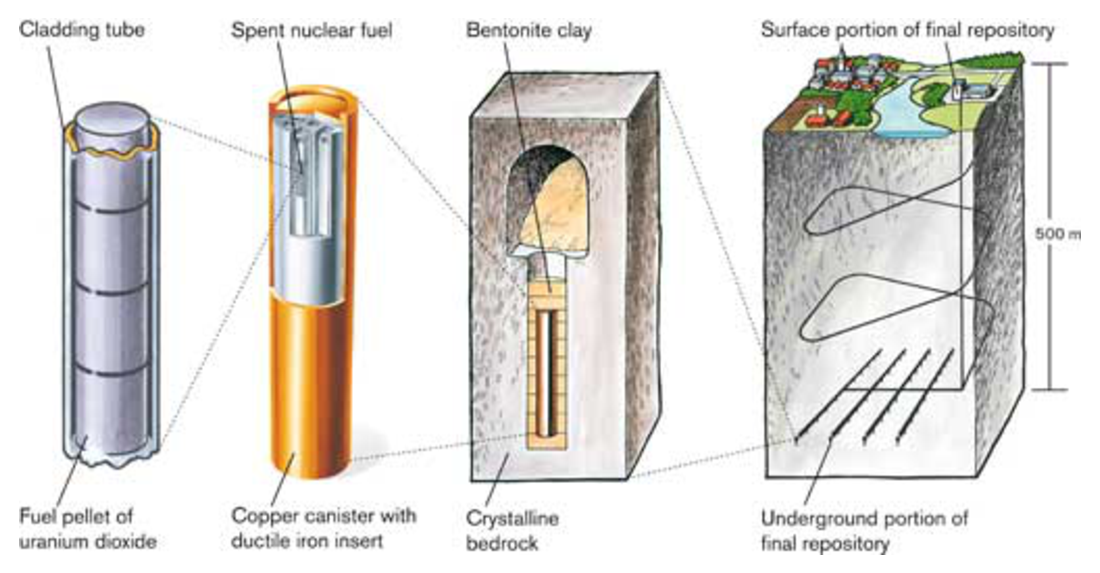
\includegraphics[width=0.7\textwidth]{./images/skb_components.eps}
  \end{center}
  \caption{Geologic disposal systems typically employ engineered barrier 
    systems as well as natural barrier systems. This is a Swedish concept in 
    granite \cite{ab_long-term_2006}.}
  \label{fig:skb_components}
\end{figure}

}
\end{frame}

%%----------------------------------------%%
\begin{frame}[ctb!]
  \frametitle{Engineered Barriers : Waste Forms}
\footnotesize{
  The first line of defense is the waste form.
  \begin{figure}[htbp!]
  \begin{center}
    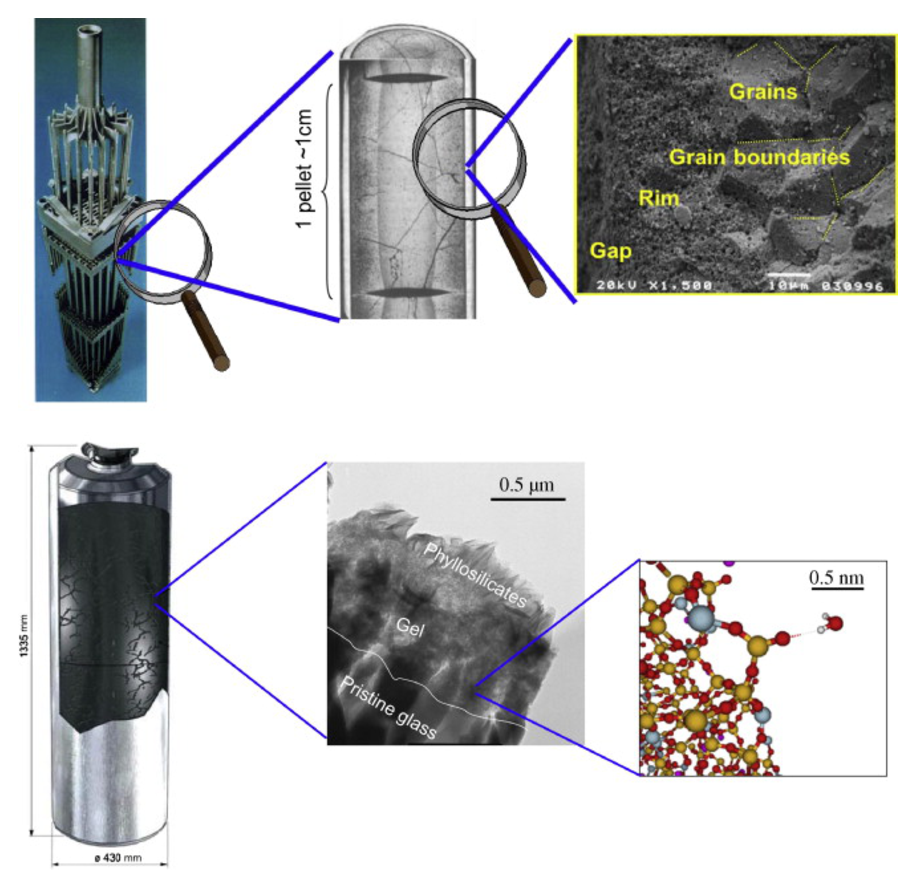
\includegraphics[width=0.5\textwidth]{./images/waste_forms_poinssot.eps}
  \end{center}
  \caption{A comparison of uranium oxide and borosilicate glass waste forms 
  \cite{poinssot_long-term_2012}.}
  \label{fig:waste_forms_poinssot}
\end{figure}

}
\end{frame}

%%----------------------------------------%%
\begin{frame}[ctb!]
  \frametitle{Engineered Barriers : Waste Packages}
\footnotesize{
  \begin{figure}[htbp!]
  \begin{center}
    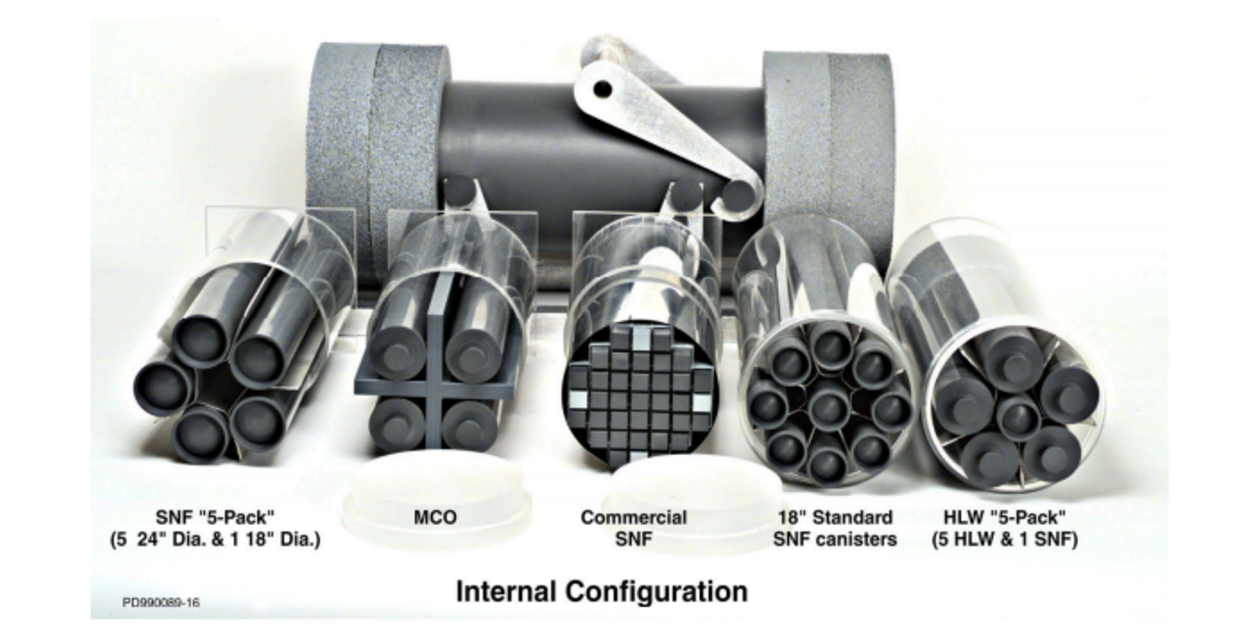
\includegraphics[width=0.7\textwidth]{./images/packages_ineel.eps}
  \end{center}
  \caption{Conceptual mockup of waste packages around waste forms 
    \cite{bridges_standardized_2001}.}
  \label{fig:packages}
\end{figure}

}
\end{frame}

%%----------------------------------------%%
\begin{frame}[ctb!]
  \frametitle{Engineered Barriers : Disposal Cask}
\footnotesize{
  \begin{figure}[htbp!]
  \begin{center}
    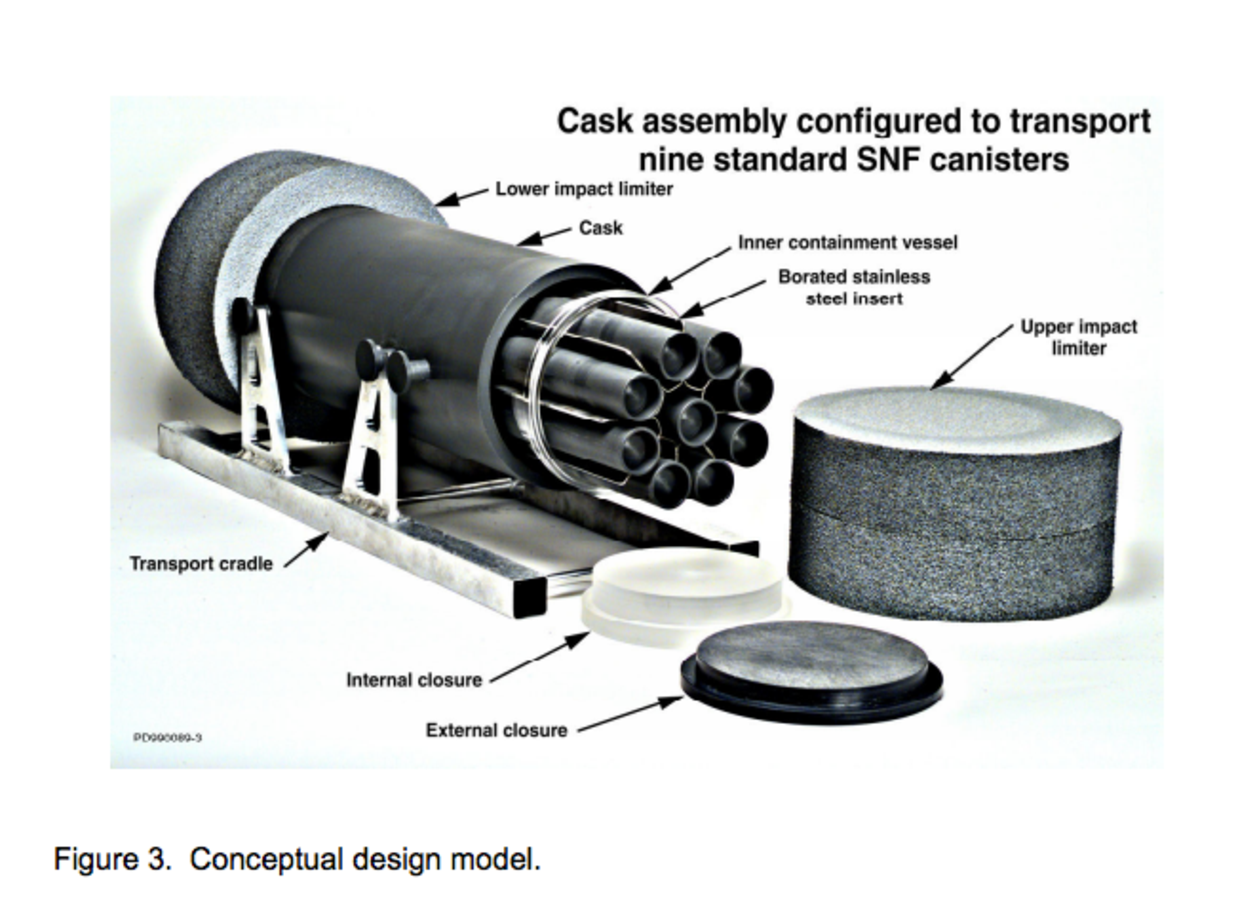
\includegraphics[width=0.7\textwidth]{./images/cask_ineel.eps}
  \end{center}
  \caption{Conceptual mockup of a transport and disposal cask 
    \cite{bridges_standardized_2001}.}
  \label{fig:packages}
\end{figure}

}
\end{frame}

%%----------------------------------------%%
\begin{frame}[ctb!]
  \frametitle{Engineered Barriers : Buffer}
\footnotesize{
  \begin{figure}[h!]
    \begin{center}
      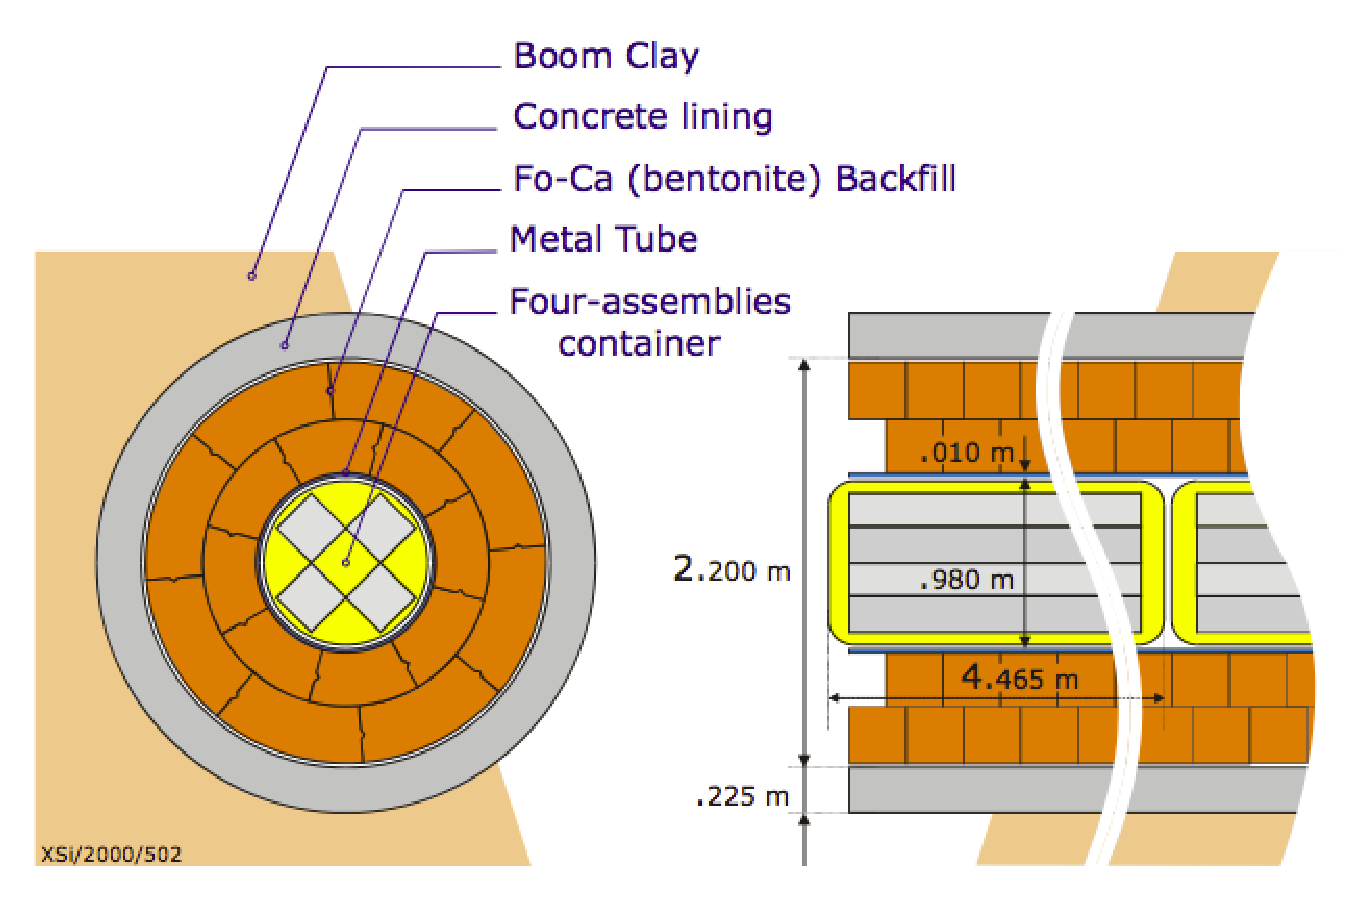
\includegraphics[height=.7\textheight]{./images/belgianClayRedImp.eps}
    \end{center}
    \caption{Belgian reference concept in Boom Clay 
    \cite{von_lensa_red-impact_2008}.}
    \label{fig:belgianClayRedImp}
  \end{figure}
}
\end{frame}

%%----------------------------------------%%
\begin{frame}[ctb!]
  \frametitle{Natural Barrier : Geology}
\footnotesize{
  \begin{figure}[htbp!]
  \begin{center}
    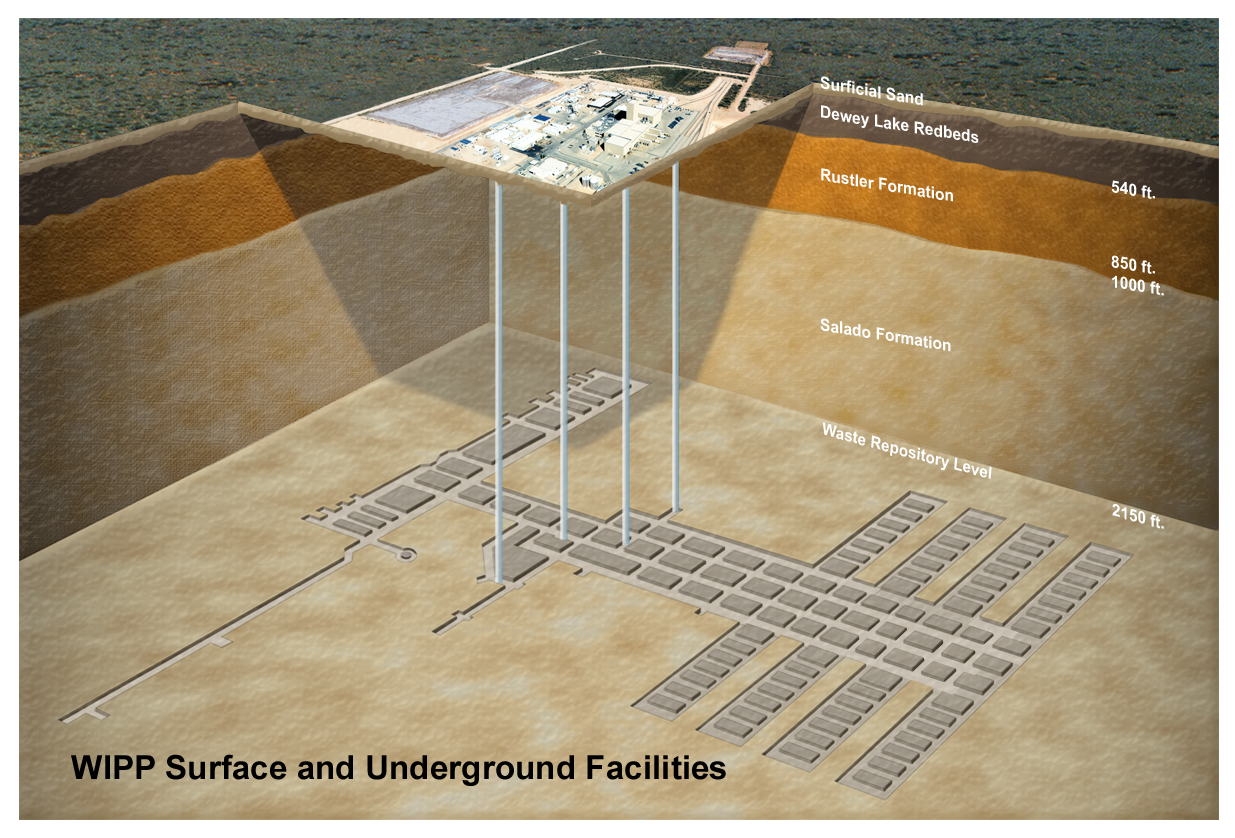
\includegraphics[width=0.7\textwidth]{./images/wipp_stratigraph.eps}
  \end{center}
  \caption{The Waste Isolation Pilot Plant has many geologic layers above the 
    salt bed \cite{doe_wipp_2013}.}
  \label{fig:wipp}
\end{figure}

}
\end{frame}

\begin{frame}
  \frametitle{Repository Layouts}

  \begin{minipage}{0.49\textwidth}
    \begin{figure}[h!]
      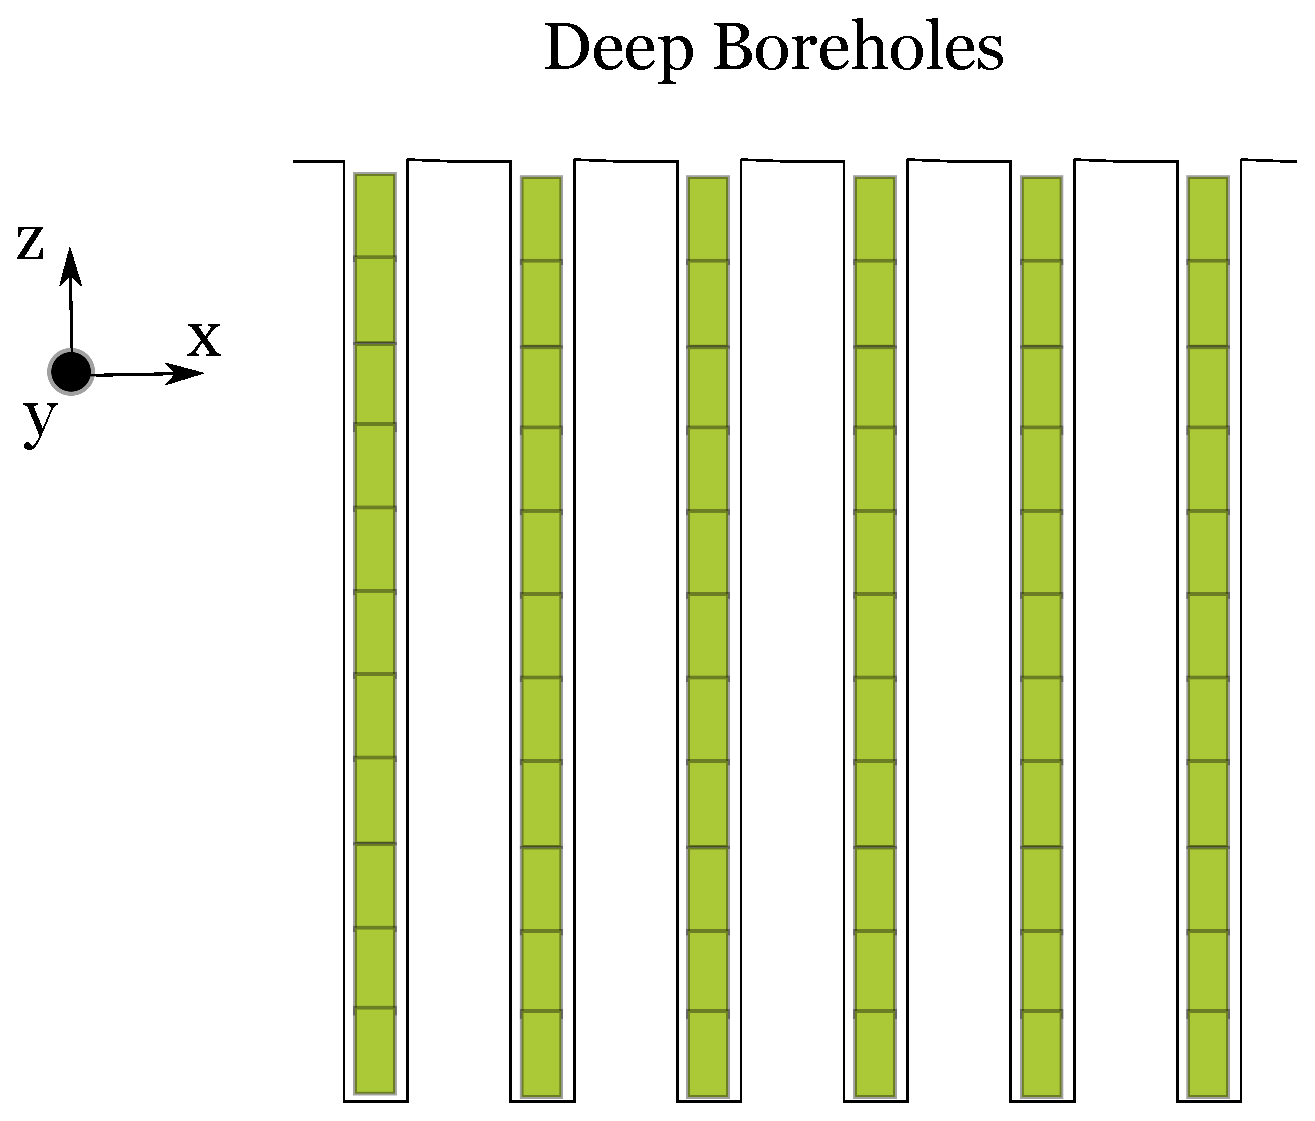
\includegraphics[width=0.75\textwidth]{./images/boreholes.eps}
    \end{figure}
    \begin{figure}[h!]
      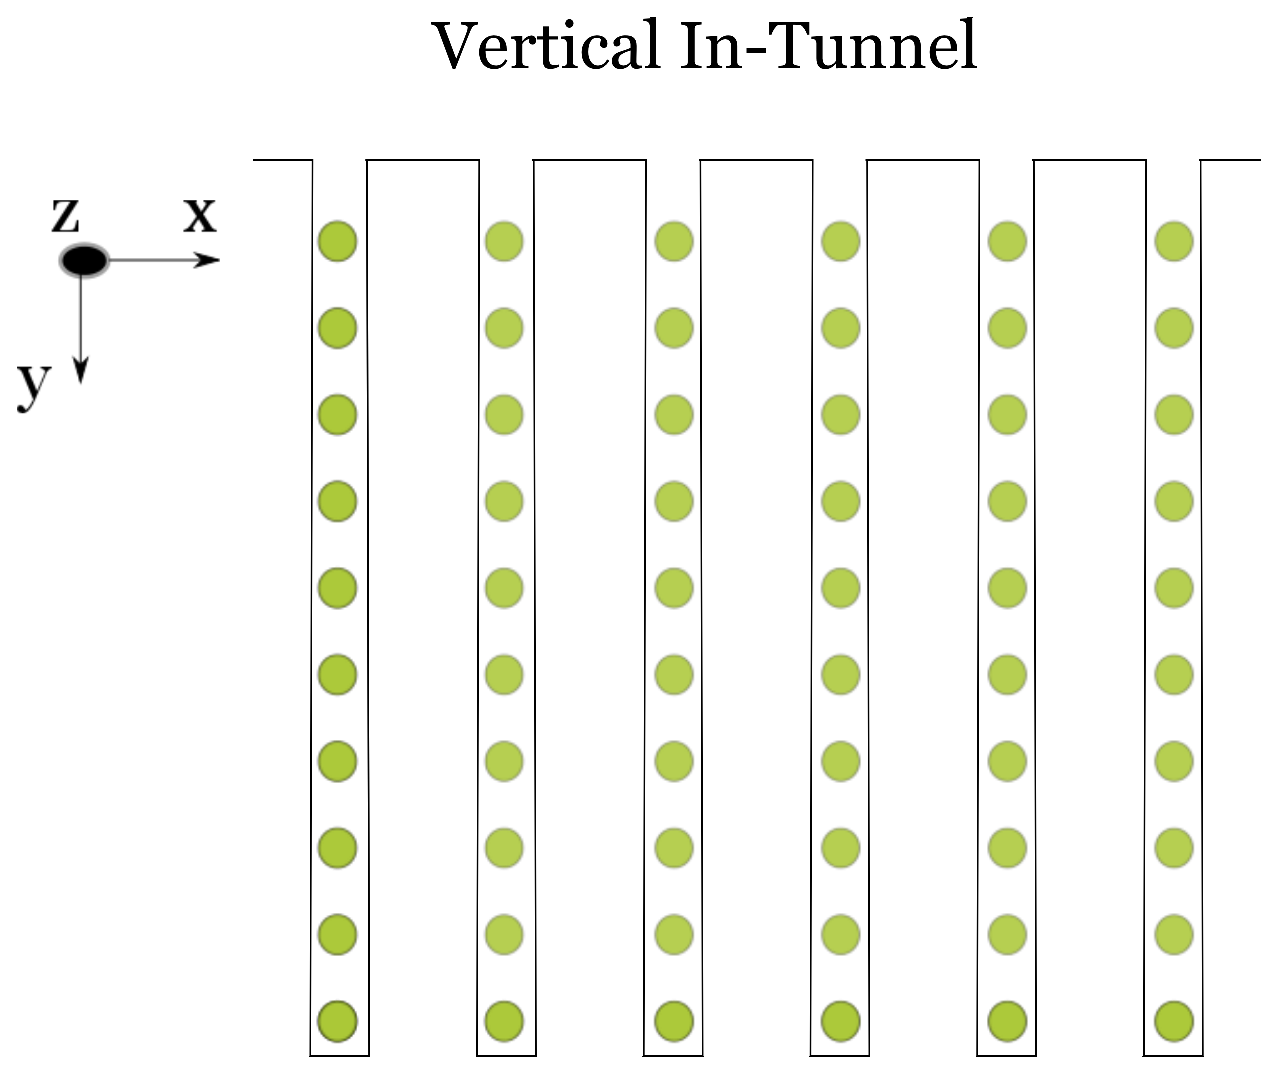
\includegraphics[width=0.75\textwidth]{./images/vertical.eps}
    \end{figure}
  \end{minipage}
  \hspace{0.01cm}
  \begin{minipage}{0.49\textwidth}
    \begin{figure}[h!]
      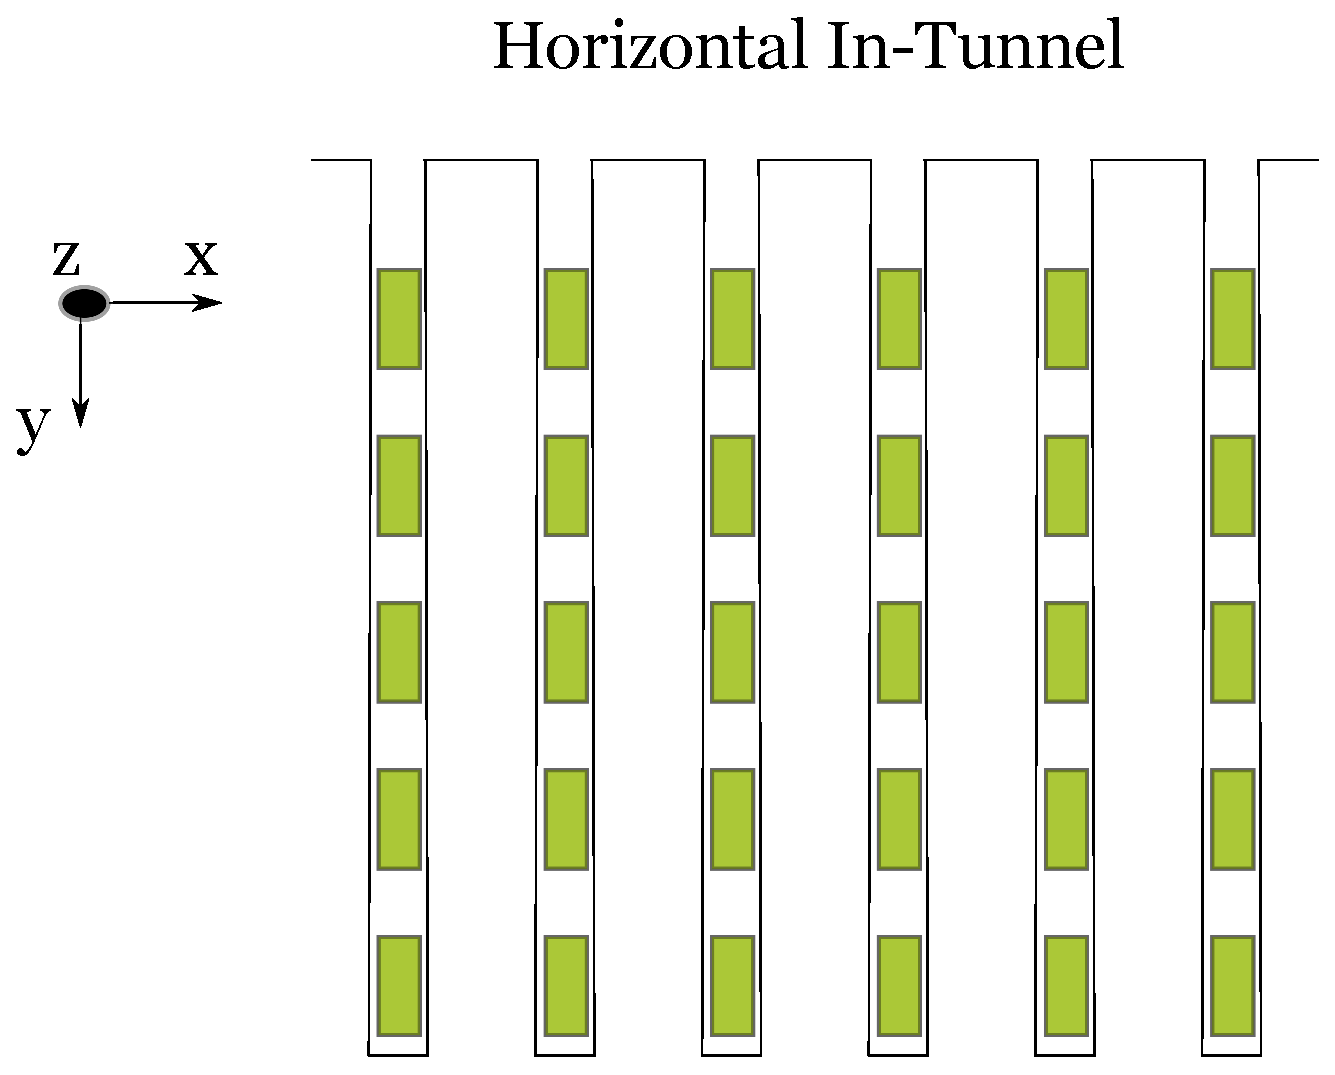
\includegraphics[width=0.8\textwidth]{./images/horizontal.eps}
    \end{figure}
    \begin{figure}[h!]
      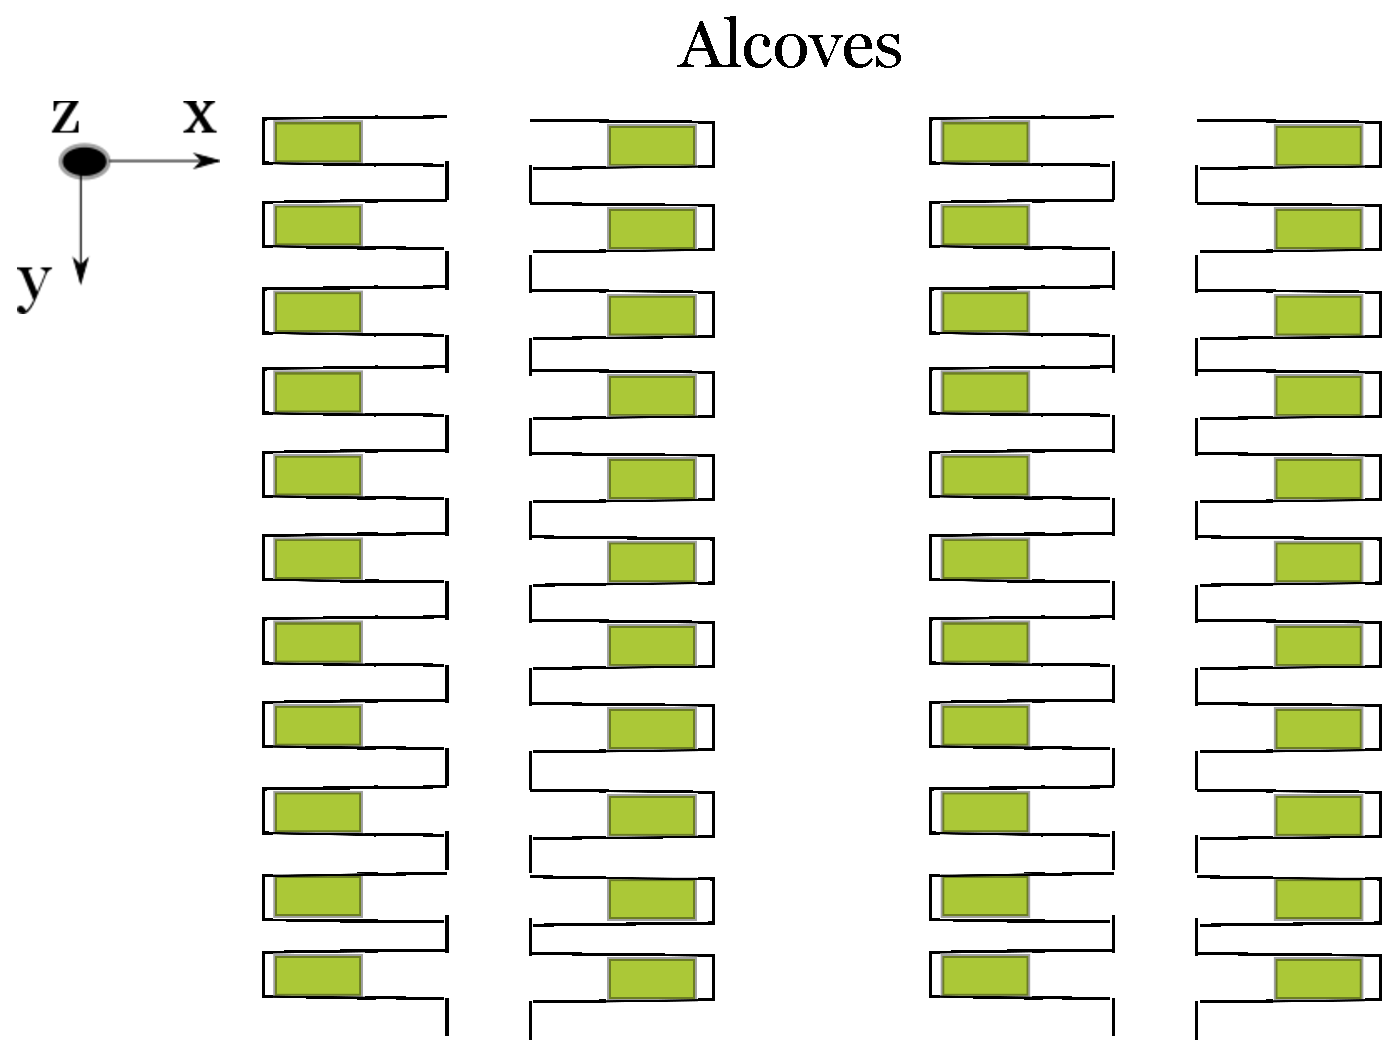
\includegraphics[width=0.8\textwidth]{./images/alcoves.eps}
    \end{figure}
  \end{minipage}

\end{frame}

\begin{frame}[ctb!]
  \footnotesize{
  \frametitle{Unsaturated, Ventilated Concepts}
  \begin{figure}[htbp!]
  \begin{center}
    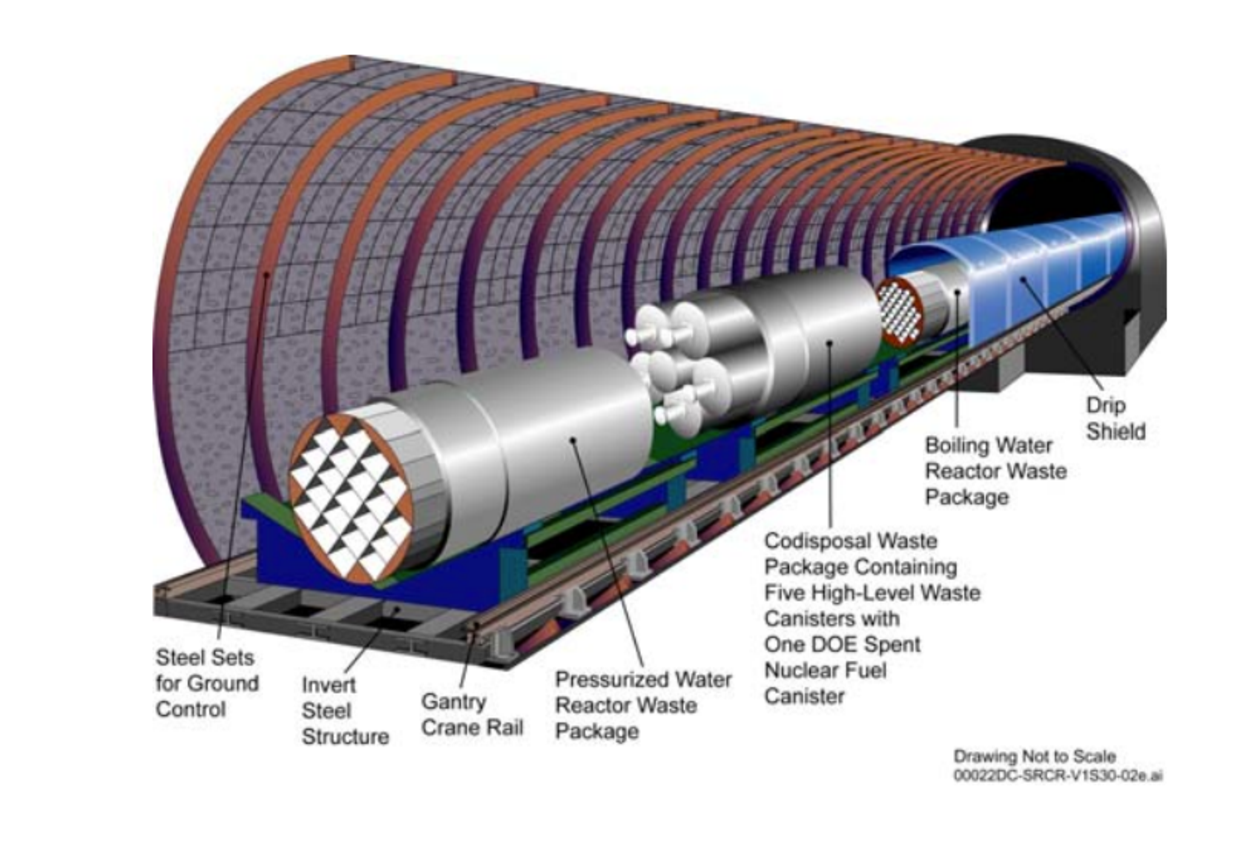
\includegraphics[height=0.7\textwidth]{./images/yucca_tunnel.eps}
  \end{center}
  \caption{The current U.S. geologic disposal concept \cite{peters_whats_2013}.}
  \label{fig:yucca_tunnel}
\end{figure}

}
\end{frame}

\begin{frame}[ctb!]
  \footnotesize{
  \frametitle{Saturated , Enclosed Concepts} 
 \begin{figure}[h!]
    \begin{center}
      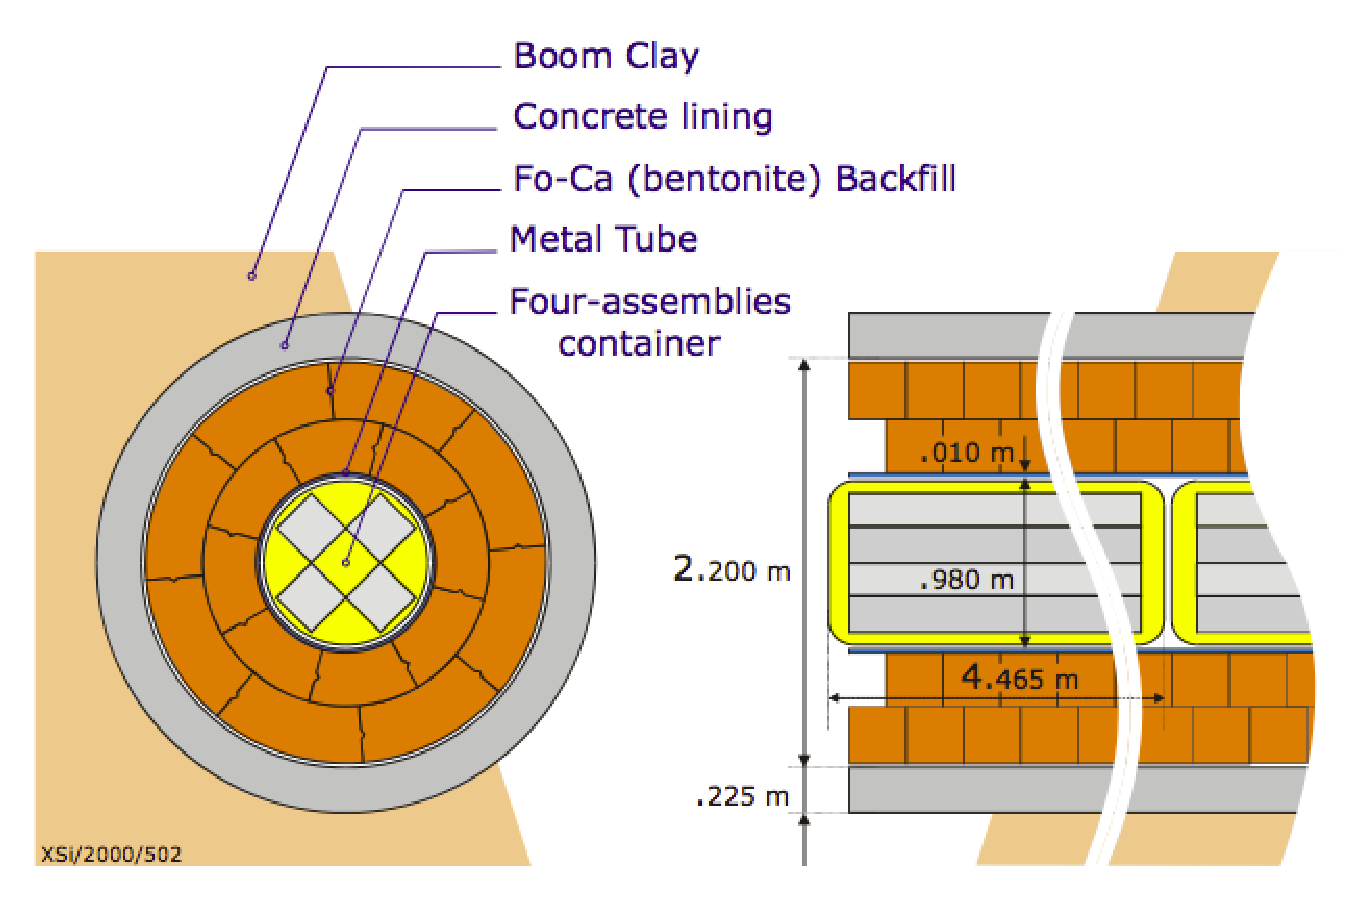
\includegraphics[height=.7\textheight]{./images/belgianClayRedImp.eps}
    \end{center}
    \caption{The Belgian reference concept in Boom Clay is backfilled very soon
   after waste emplacement without a ventilation period and is located below the water table
   \cite{von_lensa_red-impact_2008}.}
    \label{fig:belgianClayRedImp}
  \end{figure}
}
\end{frame}



\begin{frame}[ctb!]
  \frametitle{Disposal Geology Options Considered}
   \begin{minipage}{0.44\textwidth}
     \begin{figure}[h!]
         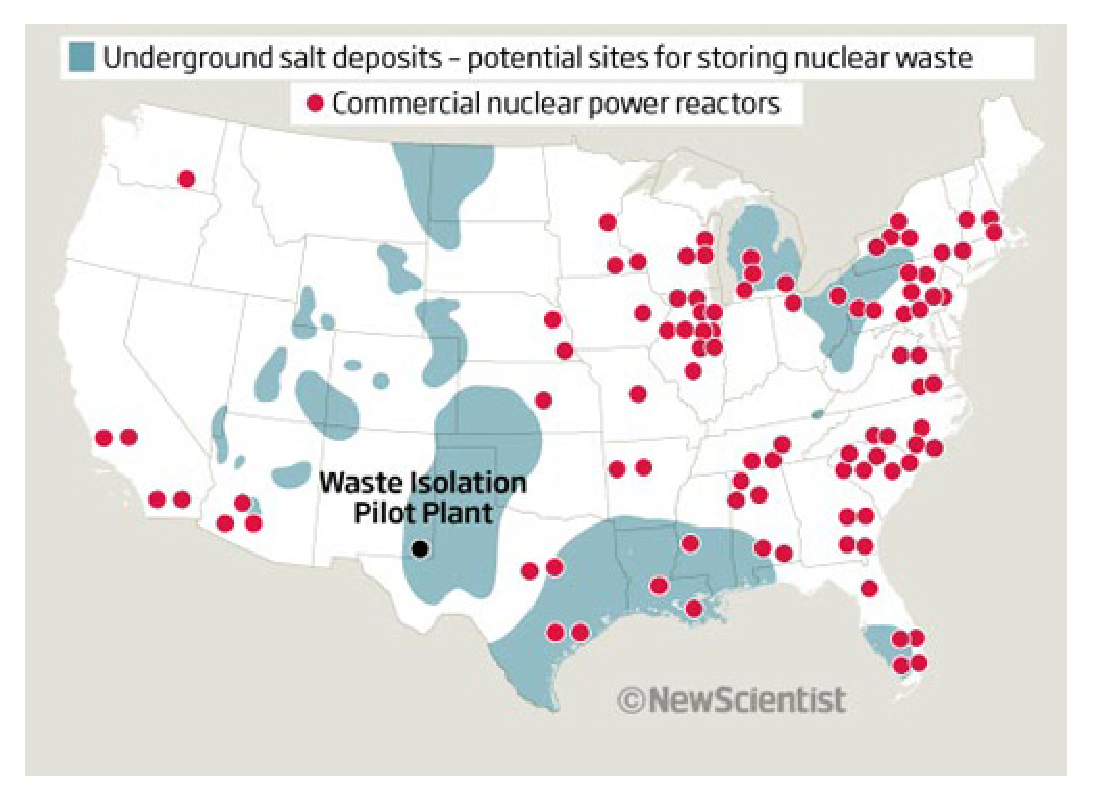
\includegraphics[width=0.7\textwidth]{./images/saltNewScientist.eps}
         \caption{U.S. Salt Deposits, ref. \cite{newscientist_where_2011}.}
     \end{figure}
     \begin{figure}[h!]
         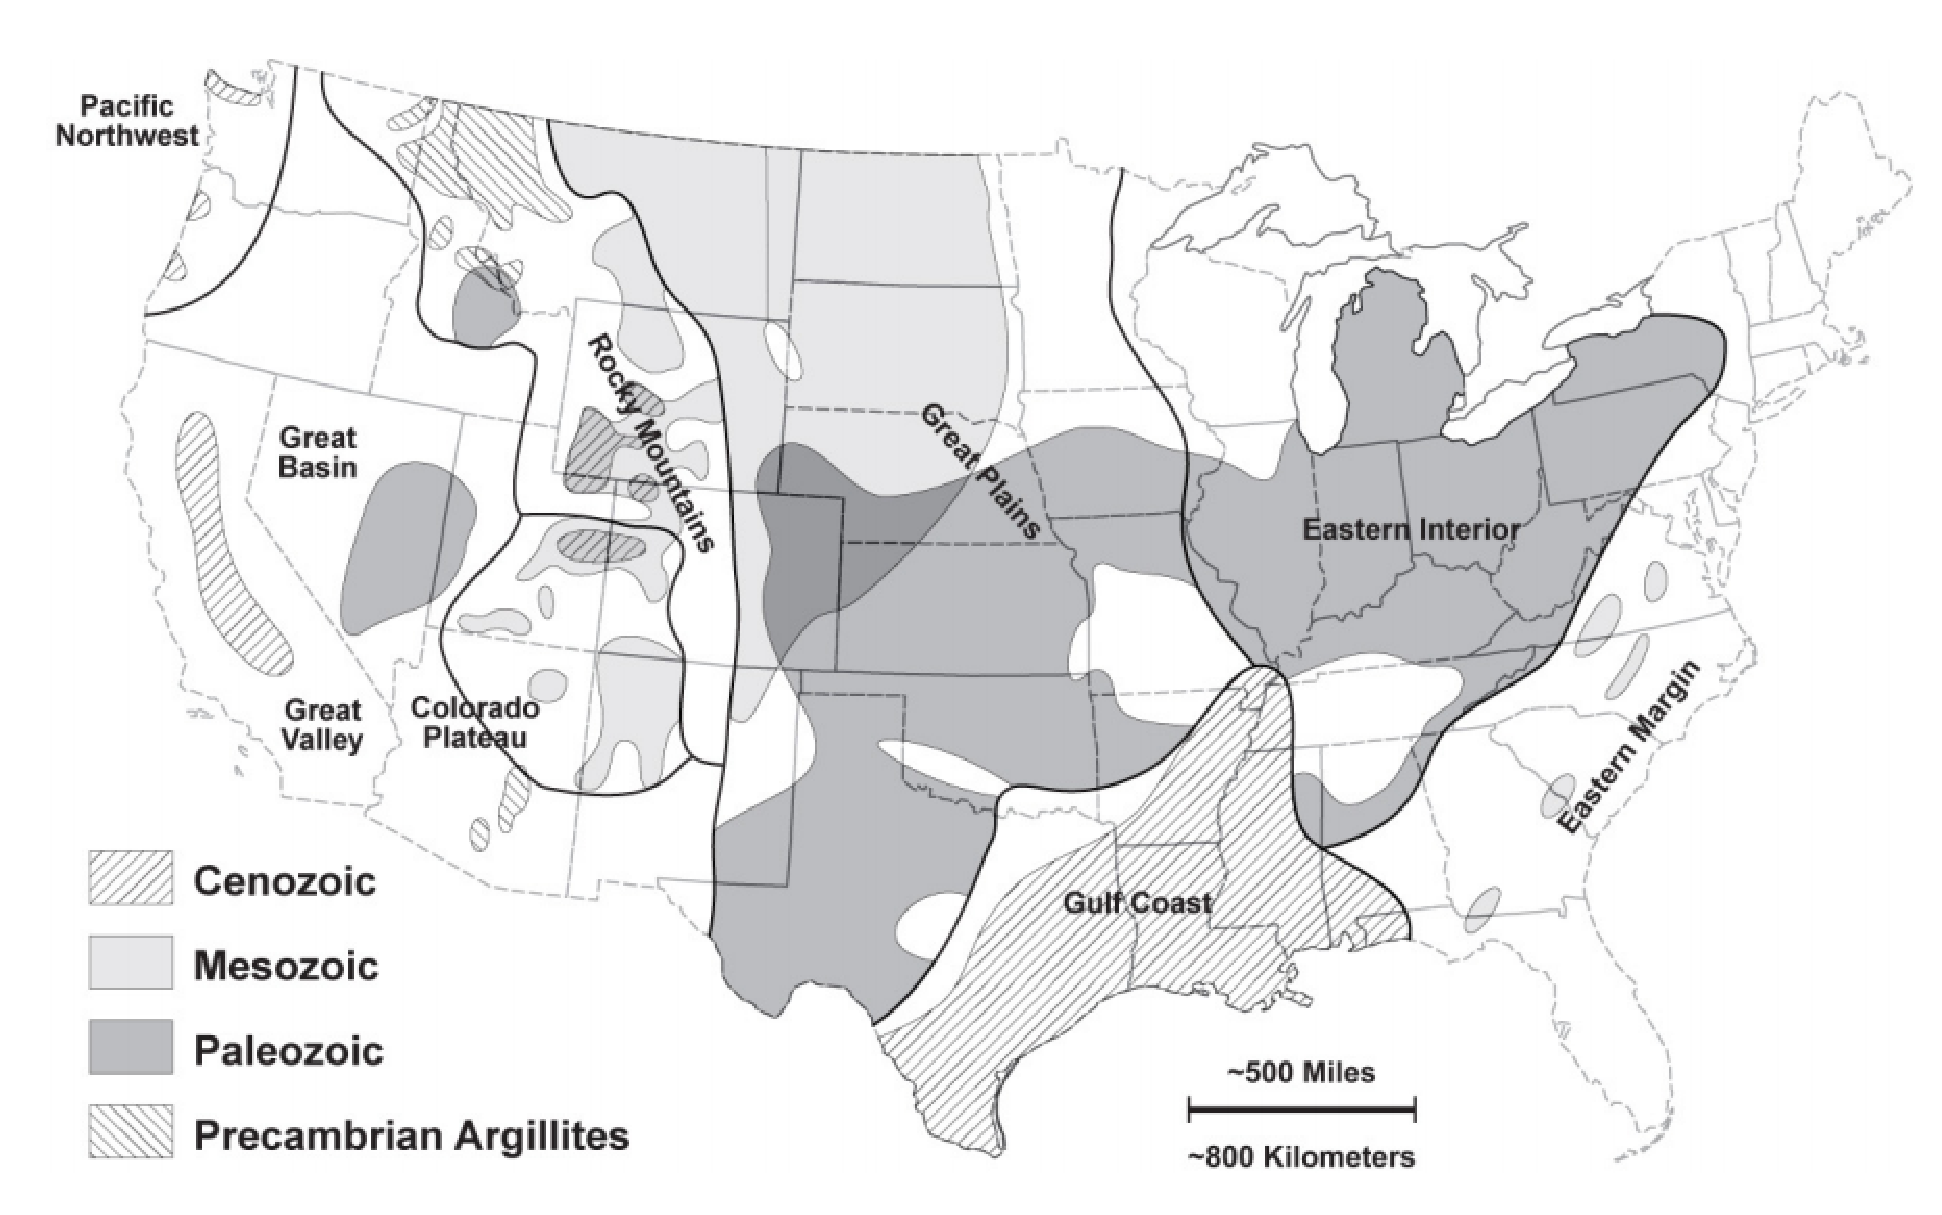
\includegraphics[width=0.7\textwidth]{./images/clayGonzales.eps}
         \caption{U.S. Clay Deposits, ref. \cite{gonzales_shales_1985}.}
     \end{figure}
   \end{minipage}
   \begin{minipage}{0.44\textwidth}
     \begin{figure}[h!]
         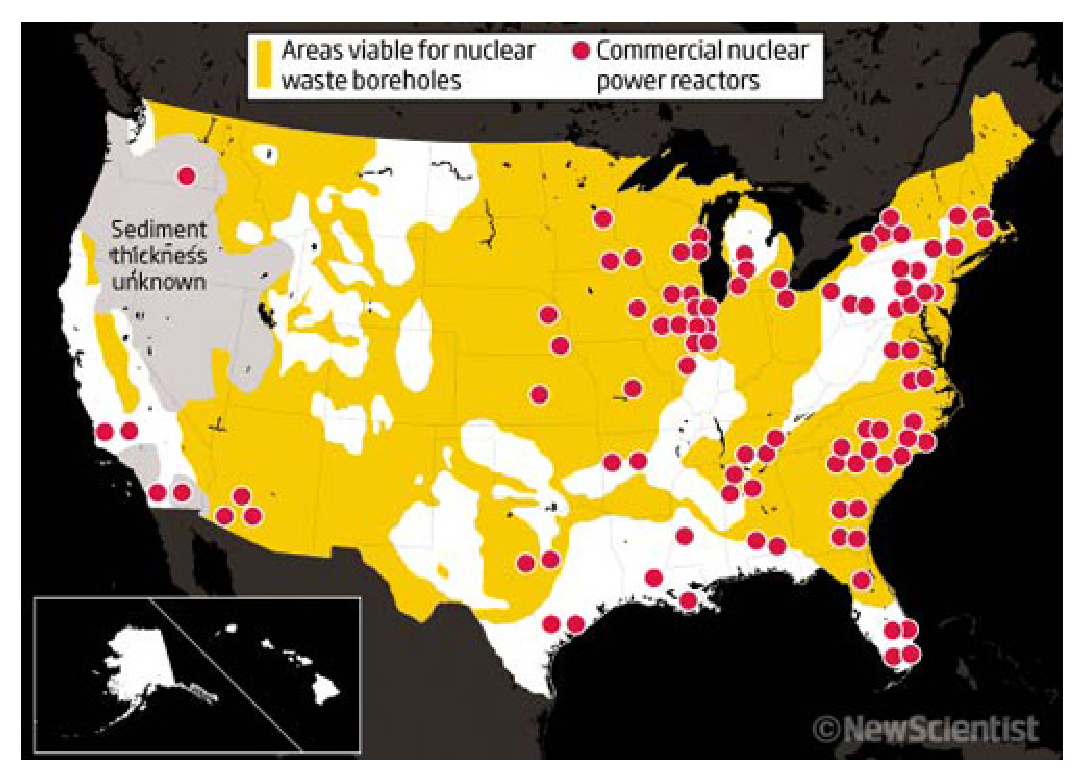
\includegraphics[width=0.7\textwidth]{./images/boreholeNewScientist.eps}
         \caption{U.S. Crystalline Basement, ref.  \cite{newscientist_where_2011}.}
     \end{figure}
     \begin{figure}[h!]
         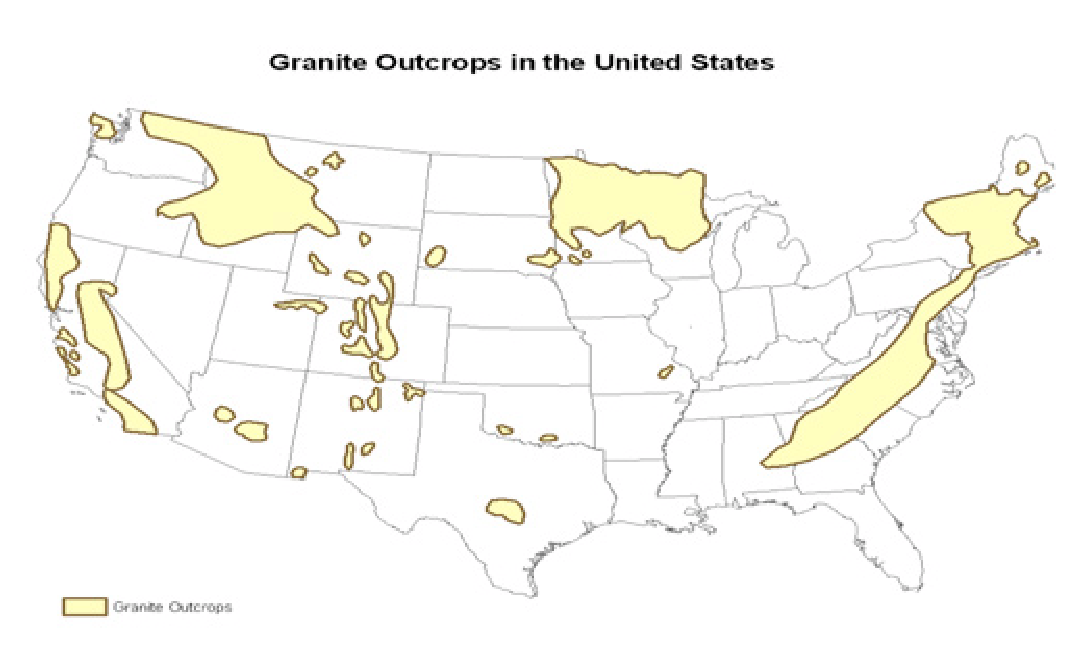
\includegraphics[width=0.7\textwidth]{./images/graniteBush.eps}
         \caption{U.S. Granite Beds, ref. \cite{bush_economic_1976}.}
     \end{figure}
   \end{minipage}
\end{frame}

\subsection{Fuel Cycle Simulator Capabilities}

\section{Geologic Repository Performance}
\subsection{Metrics}
\include{performance_metrics}
\subsection{Thermal Loading}
\include{performance_thermal}
\subsection{Radionuclide Transport and Release}
\include{performance_release}

\section{Modeling Paradigm}
\subsection{Cyclus Modeling Paradigm}
\subsection{Cyder Modeling Paradigm}


\section{Abstracted Models}
\subsection{Thermal Transport in Cyder}
\chapter{Thermal Transport Computational Models}\label{ch:thermal_models}

The results here provide an overview of the relative importance of thermal
parameters that affect the repository capacity of simplified generic
disposal concept in various geologic media where conduction is the dominant
heat transfer mode. The applicability of this sensitivity analysis is thus
restricted to enclosed, backfilled concepts.  

\subsection{Parametric Domain}

Sensitivity analyses were conducted which span the parametric range of values 
generated by the reference specific temperature change database and described 
in Table \ref{tab:thermal_cases}.  

\begin{table}[ht!]
\centering
\footnotesize{
\begin{tabular}{|l|l|l|r|}
\multicolumn{4}{c}{\textbf{Thermal Cases}}\\
\hline
\textbf{Parameter} & \textbf{Symbol} & \textbf{Units} & \textbf{Value Range} \\
\hline
Diffusivity & $\alpha_{th}$ & $[m^2\cdot s^{-1}]$ & $1.0\times10^{-7}-3.0\times10^{-6}$\\
\hline
Conductivity & $K_{th}$     & $[W\cdot m^{-1} \cdot K^{-1}]$ & $0.1 - 4.5$ \\
\hline
Spacing & $S$ & $[m]$ & 2, 5, 10, 15, 20, 25, 50 \\
\hline
Radius & $r_{lim}$ & $[m]$ & 0.1, 0.25, 0.5, 1, 2, 5 \\
\hline
Isotope & $i$ & $[-]$ & $^{241,243}Am,$  \\
        & & & $^{242,243,244,245,246}Cm,$  \\
        & & & $^{238,240,241,242}Pu$  \\
        & & & $^{134,135,137}Cs$  \\
        & & & $^{90}Sr$  \\
\hline
\end{tabular}
\caption{A thermal reference dataset of \gls{STC} values as a function of each of these parameters was generated by repeated parameterized runs of the LLNL 
MathCAD model\cite{greenberg_application_2012, greenberg_investigations_2012}.}
\label{tab:thermal_cases}
}
\end{table}



These values were selected to provide detail in the near field and at values of
$\alpha_{th}$ and $K_{th}$ in the three host media under consideration in this
work.

\subsection{Approach}

% used existing gdsms 
This analysis utilized the \gls{LLNL} semi-analytic MathCAD model
discussed in Section \ref{sec:llnl_background}.  It performs detailed
calculations of the conductive thermal transport in a generic repository
concept with a gridded layout.  

It relies on the thermal diffusivity, $\alpha_{th}$ and conductivity $K_{th}$ of 
the material as well as the waste package spacing, $S$, and thermally limiting 
radius, $r_{lim}$. Finally, it relies on the \gls{STC} data calculated with the 
semi-analytic model based on the decay heat profiles of the emplaced wastes, $Q$. 
The essential decay heat profiles, $Q$, were retrieved from a \gls{UFD} database 
provided by Carter et al. \cite{carter_fuel_2011}.



\subsection{Thermal Capacity Approximation Methodology}\label{sec:capacity}

\subsubsection{Lumped Parameter Radionuclide Mass Balance Model}\label{sec:lumped}

For systems in which the flow is sufficiently slow to be assumed constant over 
a time step, it is possible to model a system of volumes as a connected lumped 
parameter models (Figure \ref{fig:lumpedseries}). 
The Lumped Parameter mass balance model implements a response function model 
based on this lumped parameter interpretation and capable of Piston Flow, 
Exponential, and Dispersion response functions from Maloszewski and Zuber 
\cite{maloszewski_lumped_1996}.

\begin{figure}[htbp!]
  \begin{center}
    \def\svgwidth{.8\textwidth}
    \input{./chapters/methodology/nuclide_models/mass_balance/lumped/lumpedseries.eps_tex}
  \end{center}
  \caption{A system of volumes can be modeled as lumped parameter models in 
  series.}
  \label{fig:lumpedseries}
\end{figure}

Each lumped parameter component is modeled according to a 
relationship between the incoming concentration, $C_{in}(t)$, and the outgoing 
concentration, $C_{out}(t)$, 

\begin{align}
  C_{out}(t) &= \int_0^\infty C_{in}(t-t')g(t')e^{-\lambda t'}dt'
  \label{lumped2}
  \intertext{where}
  t'  &= \mbox{ transit time }[s]\nonumber\\
  g(t')  &= \mbox{ response function, a.k.a. transit time distribution}[-]\nonumber]\\
  \lambda &= \mbox{ radioactive decay constant }[s^{-1}].\nonumber
\end{align}

Selection of the response function is usually based on experimental tracer 
results in the medium at hand. If such data is available, functions used 
commonly in chemical engineering applications \cite{maloszewski_lumped_1996} 
include the Piston Flow Model (PFM), 

\begin{align}
  g(t') &= \delta{(t'-t_t))}
  \intertext{ the Exponential Model (EM) }
  g(t') &= \frac{1}{t_t}e^{-\frac{t'}{t_t}}
  \intertext{ and the Dispersion Model (DM), }
  g(t') &= \left( \frac{\emph{Pe }t_t}{4\pi t'} \right)^{\frac{1}{2}}
  \frac{1}{t'}e^{- \frac{\emph{Pe }t_t\left( 1- \frac{t'}{t_t}  \right)^2} 
  {4t'}}, \intertext{where}
  \emph{Pe}  &= \mbox{ Peclet number for mass diffusion }[-]\nonumber\\
  t_t  &= \mbox{ mean tracer age }[s]\nonumber\\
    &= t_w \mbox{ if there are no stagnant areas }\nonumber\\
  t_w  &= \mbox{ mean residence time of water }[s]\nonumber\\
       &= \frac{V_m}{Q}\nonumber\\
       &= \frac{z}{v_z}\nonumber\\
       &= \frac{z\theta_e}{q}\nonumber
  \intertext{in which}
  V_m  &= \mbox{ mobile water volume }[m^3]\nonumber\\
  Q    &= \mbox{ volumetric flow rate }[m^3/s]\nonumber\\
  z    &= \mbox{ average travel distance in flow direction }[m]\nonumber\\
  v_z  &= \mbox{ mean water velocity}[m/s]\nonumber\\
  q    &= \mbox{ Darcy Flux }[m/s]\nonumber\\
  \theta_e &= \mbox{ effective (connected) porosity }[\%].\nonumber
\end{align}

The latter of these, the Dispersion Model satisfies the one dimensional 
advection-dispersion equation, and is therefore the most physically relevant for 
this application. The solutions to these for constant concentration at the 
source boundary are given in Maloszewski and Zuber \cite{maloszewski_lumped_1996}, 

\begin{align}
  C_{out}(t) &=\begin{cases}
    PFM & C_0e^{-\lambda t_t}\\
    EM  & \frac{C_0}{1+\lambda t_t}\\
    DM & C_0e^{\frac{\emph{Pe}}{2}\left(1-\sqrt{1+\frac{4\lambda 
    t_t}{\emph{Pe}}}\right)}.
  \end{cases}
  \label{lumpedsolns}
\end{align}

Since \Cyclus handles decay outside of \Cyder, the use of these models relies on a 
reference transit time and decay constant supplied by the user. The behavior of 
the reference isotope, in this way, fully defines the behavior of all isotopes.

It is important to note that a linear concentration profile is assumed between 
the inlet and the outlet,

\begin{align}
  C(z,t) = C_{in}(t)  + \frac{C_{out}(t) - C_{in}(t)}{z_{out} - z_{in}}z.
\end{align}



\subsection{Radionuclide Transport in Cyder}

\section{Radionuclide Mass Transfer In \textsc{Cyder}}\label{sec:nuclide_models}

The results here provide an overview of the relative importance of thermal
parameters that affect the repository capacity of simplified generic
disposal concept in various geologic media where conduction is the dominant
heat transfer mode. The applicability of this sensitivity analysis is thus
restricted to enclosed, backfilled concepts.  

\subsection{Parametric Domain}

Sensitivity analyses were conducted which span the parametric range of values 
generated by the reference specific temperature change database and described 
in Table \ref{tab:thermal_cases}.  

\begin{table}[ht!]
\centering
\footnotesize{
\begin{tabular}{|l|l|l|r|}
\multicolumn{4}{c}{\textbf{Thermal Cases}}\\
\hline
\textbf{Parameter} & \textbf{Symbol} & \textbf{Units} & \textbf{Value Range} \\
\hline
Diffusivity & $\alpha_{th}$ & $[m^2\cdot s^{-1}]$ & $1.0\times10^{-7}-3.0\times10^{-6}$\\
\hline
Conductivity & $K_{th}$     & $[W\cdot m^{-1} \cdot K^{-1}]$ & $0.1 - 4.5$ \\
\hline
Spacing & $S$ & $[m]$ & 2, 5, 10, 15, 20, 25, 50 \\
\hline
Radius & $r_{lim}$ & $[m]$ & 0.1, 0.25, 0.5, 1, 2, 5 \\
\hline
Isotope & $i$ & $[-]$ & $^{241,243}Am,$  \\
        & & & $^{242,243,244,245,246}Cm,$  \\
        & & & $^{238,240,241,242}Pu$  \\
        & & & $^{134,135,137}Cs$  \\
        & & & $^{90}Sr$  \\
\hline
\end{tabular}
\caption{A thermal reference dataset of \gls{STC} values as a function of each of these parameters was generated by repeated parameterized runs of the LLNL 
MathCAD model\cite{greenberg_application_2012, greenberg_investigations_2012}.}
\label{tab:thermal_cases}
}
\end{table}



These values were selected to provide detail in the near field and at values of
$\alpha_{th}$ and $K_{th}$ in the three host media under consideration in this
work.

\subsection{Approach}

% used existing gdsms 
This analysis utilized the \gls{LLNL} semi-analytic MathCAD model
discussed in Section \ref{sec:llnl_background}.  It performs detailed
calculations of the conductive thermal transport in a generic repository
concept with a gridded layout.  

It relies on the thermal diffusivity, $\alpha_{th}$ and conductivity $K_{th}$ of 
the material as well as the waste package spacing, $S$, and thermally limiting 
radius, $r_{lim}$. Finally, it relies on the \gls{STC} data calculated with the 
semi-analytic model based on the decay heat profiles of the emplaced wastes, $Q$. 
The essential decay heat profiles, $Q$, were retrieved from a \gls{UFD} database 
provided by Carter et al. \cite{carter_fuel_2011}.




%\subsection{Mass Transfer Modes}\label{sec:mass_transfer}

\subsubsection{Calculation of Mass Transfer}
The MixedCell model can operate in four modes, each dictating the method by 
which mass transfer across the inner boundary is calculated.  Those modes 
utilize the source term, Dirichlet, and Neumann interfaces to model prescribed, 
flow, advective flow, or diffusive flow.
Once calculated, that material object is removed from the 
internal component ($m_{ij} = -\dot{m}_i$) such that its internal state can be 
queried accurately in future timesteps.  

For the case in which source term is used on the inner boundary, the mass 
transferred from component $i$ to component $j$ in timestep $t_{n}$ is simply

\begin{align} 
m_{ij} &=  \mathcal{S}_i(t_n) \nonumber
\intertext{where}
\mathcal{S}_i(t_n) &= \mbox{ source term provided by component i at }t_n [kg].
\end{align}

For the case in which Dirichlet is used, the mass transferred is determined by 
advection. One dimensional mass flux due to advection is the speed of flowing 
water, $v_z$, scaled by the concentration of contaminants fixed by the Dirichlet 
boundary condition, $C$, all integrated over the porous, degraded area perpendicular to 
the flow, $\theta dxdy$,

\begin{align}
  m_{ij} &= \int_{t_{n-1}}^{t_n}\int_0^y\int_0^x\theta d v_z \mathcal{D}_i(t_n) dxdydt \label{mixed_adv}
\intertext{which, for the Cyder components, becomes }
m_{ij} &= \theta d v_z C 2rl (t_n - t_{n-1})\nonumber\\
\intertext{where}
\mathcal{D}_i(t_n) &= \mbox{ fixed C from component i at }t_n [kg/m^3]\nonumber\\
r &= \mbox{ radius of the cylinder }[m]\nonumber\\
l &= \mbox{ length of the cylinder }[m].\nonumber
\end{align}

For the case in which Neumann is chosen, the mass transfer is taken to be 
dispersive, 

\begin{align}
  m_{ij} &= \int_{t_{n-1}}^{t_n}\int_0^y\int_0^x -D \theta d \mathcal{N}_i(t_n) dxdydt \label{mixed_adv}\\
         &= \int_{t_{n-1}}^{t_n}\int_0^y\int_0^x -D \theta d \frac{\partial C}{\partial z}\Bigg|_{z=r_j} dxdydt \nonumber
\intertext{which, for the Cyder components, becomes }
m_{ij} &= -D \theta d \frac{\partial C}{\partial z}\Bigg|_{z=r_j} 2rl(t_n - t_{n-1}).\nonumber
\end{align}

\subsubsection{Boundary Interfaces}
The source term of available contaminants is all mass in the available degraded fluid,
\begin{align}
\mathcal{S}_j(t_n) &= m_{df}(t_n). 
\end{align}
The desired boundary conditions can be expressed in terms of $m_{df}$. First, the 
Dirichlet boundary condition is 
\begin{align}
\mathcal{D}_j(t_n) &= C_j(t_n)\nonumber\\ 
 &= \frac{m_{df}(t_n)}{V_{df}(t_n)}.
\label{dirichlet_mixed}
\end{align}

From this boundary condition in combination with global advective velocity 
data, porosity data,  and elemental dispersion coefficient data, all other 
boundary conditions can be found. The Neumann boundary condition generated at 
the external boundary of cell $j$ relies on up to date data from cell $k$ and 
on internal state data from the previous time step, such that 

\begin{align}
\mathcal{N}_j(t_n)&= \frac{dC(t_n)}{dr}\Bigg|_{r=r_j}\nonumber\\ 
                  &= \frac{C_k(r_{k-1/2},t_{n-1}) - C_i(r_{j-1/2}, t_n)}{r_{k-1/2} - r_{j-1/2}}
\label{neumann_mixed}
\intertext{where}
r_{j-1/2} &= r_{j} - \frac{r_{j} - r_{i}}{2}.\nonumber\\
r_{k-1/2} &= r_{k} - \frac{r_{k} - r_{j}}{2}.\nonumber
\end{align}

This expression for the concentration gradient can also be used in the Cauchy 
boundary condition, which relies on the advective velocity and concentration 
profile as well as the concentration gradient,

\begin{align}
v_z C_0 &= \frac{dC(t_n)}{dr}\Big|_{r=r_{j}} + v_{z}C_j(t_n).
\label{cauchy_mixed}
\end{align}


%\subsection{Time Step Algorithm}\label{sec:timestep}
\subsection{Time Stepping Algorithm}\label{sec:time stepping}

In \Cyder, radionuclide contaminant flow is assumed to travel outward from 
the central Component (and up, in the $\hat{k}$ direction). In order to conduct 
a mass balance in each Component at each time step, the mass flow and mass 
balance calculations proceed from the innermost Component to the outermost 
Component. As mass flows from inner components to outer components, the mass 
balances in both components are updated.  Thus, nuclide release information is 
passed radially outward from the waste stream sequentially through each 
containment layer to the geosphere.  This implicit time stepping method 
arrives at the updated state of each Component, radially outward, as a function 
of both the past state and the current state of the system. 

At each component interface where mass transfer occurs and within each component 
where mass balances take place, the flow model is solved with the most up to 
date information available.  To illustrate the algorithm by which mass flow 
calculations are conducted through the system of components at each time step, we 
will walk through the phases of a single time step for a simple pair of 
components. The source, $i$, is the inner and the sink, $j$, is the outer
component. 

\subsubsection{Phase 1: Initial Conditions}

The initial conditions in both the source and the sink at the beginning of a 
time step are equal to the final updated state of the previous time step. If this 
is the first time step, the global intial state of the repository system is used. 

\subsubsection{Phase 2: Interior Mass Balance}

The mass distrubution and concentration profile in the interior source volume 
$i$ is solved based on the initial condition, any influxes, and the physics of 
its mass balance model.  This calculation results in a contaminant mass 
distribution and concentration profile within the volume $i$ at time $t_n$.  
For each of the models, the calculation behind this mass distribution and 
concentration profile is disscussed in Section \ref{sec:mass_balance}.

This mass distribution and concentration profile fully inform 
the conditions on the boundary at $r_i$ and this information is made available 
to the external component, $j$.


\subsubsection{Phase 3: Mass Transfer Calculation}

The mass transfer from the source volume $i$ to the sink volume $j$ is 
calculated next, based on the up to date conditions at $0\le r \le r_{i}$ 
determined in Phase 2 and the initial conditions in volume $j$ where $r_i \le r 
\le r_j$. The mass transfer is calculated according to the mass transfer mode 
preference of the mass balance model of volume $j$.  

The Degradation Rate and Mixed Cell models can be parameterized to utilize an 
explicit mass transfer mode that captures either advection, dispersion, or 
coupled flow.  The Lumped Parameter and One Dimensional PPM models, on the 
other hand, use an implcit method by which the incoming mass flux is determined 
based on the expected concentration profile resulting from the internal 
Dirichlet boundary condition at $r_i$. 

\subsubsection{Phase 4: Exterior Mass Balance}

When a mass flux $m_{ij}(t_n)$ is determined between volumes $i$ and $j$, the 
mass is added to the exterior sink volume $j$. Accordingly, necessary updates 
are made to the mass balance and concentration profile.  For each of the 
models, the calculation behind this mass distribution and concentration profile 
is disscussed in Section \ref{sec:mass_balance}.

\subsubsection{Phase 5: Interior Mass Balance Update}

When a mass flux $m_{ij}(t_n)$ is determined between volumes $i$ and $j$, the 
mass is simultanously added to the exterior sink volume $j$ (as in phase 4) and 
extracted from the interior source volume $i$.  When the material is extracted 
from the interior source volume, the contained mass distribution and 
concentration profile are updated to reflect this change.  

\subsubsection{old text}


That is, in Component $j$, some Component in a nested series, the mass flux 
entering the Component at time $t_n$ is found from the initial state of the cell 
at time $t_n$, the inner boundary 
condition at time $t_n$ and the outer boundary condition at $t_{n-1}$.  

\begin{align}
  \dot{m}_{ij}^n &= f( m_j(t_{n-1}) , BC_i(t_n) , BC_j(t_{n-1}) . . . ) \nonumber\\
  \intertext{where}
  m_{ij}(t_n) &= \mbox{ contaminant mass flux from component i to j }[kg/time step]\nonumber\\
  BC_i(t_n)  &= \mbox{ inner conditions at }r_i\mbox{, and time }t_n \nonumber \\
  BC_j(t_{n-1})  &= \mbox{ outer conditions at }r_j\mbox{, and time }t_{n-1} \nonumber\\
  f &= \mbox{ functional form of contaminant transport into j. }\nonumber
\end{align}

Once the mass flux into the component is found, the mass is removed from the 
inner cell, updating its state in preparation for the next time step.

\begin{align}
  m_i^\dagger(t_n)  &= m_i(t_n)  - m_{ij}(t_n) 
  \intertext{where}
  m_i^\dagger(t_n)  &= \mbox{ updated mass in component i }[kg]
\end{align}

In this way, the contained mass in the component is described as
\begin{align}
  m_j(t_n)  &= m_j(t_{n-1})  + \dot{m}_j(t_n) . \nonumber
\end{align}

Resulting concentration profiles across the component can then be calculated 
and one can solve, numerically, for the outer boundary condition at $t_n$ 

\begin{align}
  BC_j(t_n) &= g\left( m_j(t_n) , C_j(t_n) \right)\nonumber\\
  g &= \mbox{functional form of contaminant transport across j}\nonumber
\end{align}

This boundary condition can, in turn, be used by the component external to it, $k$ as the $t_n$ 
inner boundary condition of its own solution and so on.



%\subsection{Mass Inventory and Distribution Models}\label{sec:mass_balance}

The results here provide an overview of the relative importance of thermal
parameters that affect the repository capacity of simplified generic
disposal concept in various geologic media where conduction is the dominant
heat transfer mode. The applicability of this sensitivity analysis is thus
restricted to enclosed, backfilled concepts.  

\subsection{Parametric Domain}

Sensitivity analyses were conducted which span the parametric range of values 
generated by the reference specific temperature change database and described 
in Table \ref{tab:thermal_cases}.  

\begin{table}[ht!]
\centering
\footnotesize{
\begin{tabular}{|l|l|l|r|}
\multicolumn{4}{c}{\textbf{Thermal Cases}}\\
\hline
\textbf{Parameter} & \textbf{Symbol} & \textbf{Units} & \textbf{Value Range} \\
\hline
Diffusivity & $\alpha_{th}$ & $[m^2\cdot s^{-1}]$ & $1.0\times10^{-7}-3.0\times10^{-6}$\\
\hline
Conductivity & $K_{th}$     & $[W\cdot m^{-1} \cdot K^{-1}]$ & $0.1 - 4.5$ \\
\hline
Spacing & $S$ & $[m]$ & 2, 5, 10, 15, 20, 25, 50 \\
\hline
Radius & $r_{lim}$ & $[m]$ & 0.1, 0.25, 0.5, 1, 2, 5 \\
\hline
Isotope & $i$ & $[-]$ & $^{241,243}Am,$  \\
        & & & $^{242,243,244,245,246}Cm,$  \\
        & & & $^{238,240,241,242}Pu$  \\
        & & & $^{134,135,137}Cs$  \\
        & & & $^{90}Sr$  \\
\hline
\end{tabular}
\caption{A thermal reference dataset of \gls{STC} values as a function of each of these parameters was generated by repeated parameterized runs of the LLNL 
MathCAD model\cite{greenberg_application_2012, greenberg_investigations_2012}.}
\label{tab:thermal_cases}
}
\end{table}



These values were selected to provide detail in the near field and at values of
$\alpha_{th}$ and $K_{th}$ in the three host media under consideration in this
work.

\subsection{Approach}

% used existing gdsms 
This analysis utilized the \gls{LLNL} semi-analytic MathCAD model
discussed in Section \ref{sec:llnl_background}.  It performs detailed
calculations of the conductive thermal transport in a generic repository
concept with a gridded layout.  

It relies on the thermal diffusivity, $\alpha_{th}$ and conductivity $K_{th}$ of 
the material as well as the waste package spacing, $S$, and thermally limiting 
radius, $r_{lim}$. Finally, it relies on the \gls{STC} data calculated with the 
semi-analytic model based on the decay heat profiles of the emplaced wastes, $Q$. 
The essential decay heat profiles, $Q$, were retrieved from a \gls{UFD} database 
provided by Carter et al. \cite{carter_fuel_2011}.



%\subsubsection{Degradation Rate Mass Balance Model}\label{sec:deg_rate}
\subsection{Degradation Rate Radionuclide Transport Model}\label{sec:deg_rate}
The degradation rate model, simulating the fractional degradation of the 
material containment properties, is the simplest of implemented models and is most 
appropriate for simplistic waste package failure modeling. The fundamental 
concept is depicted in Figure \ref{fig:deg_volumes}.

\begin{figure}[h!]
  \begin{center}
    \def\svgwidth{.7\textwidth}
    \input{./chapters/methodology/nuclide_models/mass_balance/deg_rate/deg_volumes.eps_tex}
  \end{center}
  \caption[Constituents of a Degradation Rate Control Volume]{The control volume contains an 
  intact volume $V_i$ and a degraded volume, $V_d$. Contaminants in $V_d$ are 
  available for transport, while contaminants in $V_i$ are contained.}
  \label{fig:deg_volumes}
\end{figure}



The materials that constitute the engineered barriers in a saturated 
repository environment degrade over time. The implemented model of this nuclide 
release behavior is based solely on a fractional degradation rate. 
The degraded volume is a simple fraction, $d$, of the total volume, $V_T$, such 
that 
\begin{align}
V_T &= V_i + V_d
\label{deg_volumes}
\intertext{where}
V_d(t) &= d(t)V_T\nonumber\\
V_i(t) &= (1-d(t))V_T\nonumber\\
V_T &= \mbox{ total volume }[m^3]\nonumber\\
V_i(t) &= \mbox{ intact volume at time t }[m^3]\nonumber\\
V_d(t) &= \mbox{ degraded volume at time t }[m^3]\nonumber
\intertext{and}
d(t) &= \mbox{ the fraction that has been degraded by time t }[-].\nonumber
\end{align}


\subsubsection{Calculation of Mass Transfer}
In this model, the contaminants in the degraded fraction of the control volume 
are available to adjacent components. The available contaminants
$m_{ij}(t)$, at the boundary between cell $i$ to cell $j$ at time $t$ are thus

\begin{align}
\dot{m}_{ij}(t) &= f_im_i(t)
\label{deg_rate_source_cont}
\intertext{where}
\dot{m}_{ij} &= \mbox{ the rate of mass transfer from i to j }[kg/s]\nonumber\\
f_i &= \mbox{ degradation rate function in cell i }[1/s] \nonumber\\
m_i &= \mbox{ mass in cell i }[kg] \nonumber\\
t &= \mbox{ time  }[s].\nonumber
\end{align}

For a situation as in \Cyder and \Cyclus, with discrete time steps, the time steps are 
assumed to be small enough to assume a constant rate $m_{ij}$ over the course 
of the time step. This model incorporates the source term made available on the 
inner boundary into its available mass and defines the resulting boundary 
conditions at the outer boundary as solely a function of the degradation rate 
of that component.  The mass transferred between discrete times $t_{n-1}$ and 
$t_n$ is thus a simple linear function of the transfer rate in 
\eqref{deg_rate_source_cont}, 

\begin{align}
m_{ij}(t_n) &= \int_{t_{n-1}}^{t_n}\dot{m}_{ij}(t')dt' \nonumber\\
         &= f_im_i(t_{n-1})\left[t_n - t_{n-1}\right].
\label{deg_rate_source_discrete}
\end{align}

\subsubsection{Boundary Interfaces}
\label{sec:dr_bc}
The mass $m_{df}(t_n)$ is the source term at the outer boundary, 
\begin{align}
  \mathcal{S}_j(t_n) &= \mbox{ fixed source term flux at }r_j [kg]\nonumber\\ 
                     &= m_{df}(t_n).
\end{align}
Thus, for the case in which all engineered barrier components are represented by 
degradation rate models, the source term at the outermost edge will be solely
a function of the original central source and the degradation rates of the 
components. 

The concentration boundary condition must also be defined at the outer boundary 
to support parent components that utilize the Dirichlet boundary condition. For 
the degradation rate model, which incorporates no diffusion or advection, the 
concentration, $C_j$ at $r_j$, the boundary between cells $j$ and $k$, is the average 
concentration in the saturated pore volume,

\begin{align}
\mathcal{D}_j(t_n) &= \mbox{ fixed concentration from component j at }t_n [kg/m^3].\nonumber\\ 
                   &= C_{j}(t_n)\nonumber\\ 
                   &= C_{df}\nonumber\\
                   &= \frac{m_{d}(t_n)}{V_{d}(t_n)}\\
\label{deg_rate_dirichlet}\\
&= \frac{\mbox{ solute mass in degraded fluid in cell j }}{\mbox{ degraded fluid volume in cell j}}.\nonumber 
\end{align}

To support parent components that utilize the Neumann boundary condition, the 
concentration gradient can be found if the concentration and the 
radial midpoint of the external component, $k$, are specified.

\begin{align}
\mathcal{N}_j(t_n) &= \mbox{ fixed concentration gradient from component j at }t_n [kg/m^3/s]\nonumber\\
                   &= \frac{dC(t_n)}{dr}\Bigg|_{r=r_j}\nonumber\\ 
                   &= \frac{C_k(r_{k-1/2},t_{n-1}) - C_j(r_{j-1/2}, t_n)}{r_{k-1/2} - r_{j-1/2}}
\label{neumann_dr}
\intertext{where}
r_{j-1/2} &= r_{j} - \frac{r_{j} - r_i}{2}\nonumber\\
r_{k-1/2} &= r_{k} - \frac{r_{k} - r_j}{2}.\nonumber
\end{align}


To support parent components that utilize the Cauchy boundary condition, the 
degradation rate model assumes that the fluid velocity is constant across the cell 
as is the concentration. Thus, 

\begin{align}
\mathcal{C}_j(t_n) &= \mbox{ fixed concentration flux from component j at }t_n [kg/m^2/s]\nonumber\\
                   &= -D\frac{\partial C(t_n)}{\partial r}\Bigg|_{r=r_j} + v_zC(t_n)\Bigg|_{r=r_j} \\
\label{deg_rate_cauchy}
            &= v_zC_0\nonumber
\intertext{where}
            C_0 &= \mbox{ a fixed concentration }[kg/m^3].\nonumber
\end{align}

%<++> &= \mbox{ <++> }[<++>] \nonumber\\


%\subsubsection{Mixed Cell Mass Balance Model}\label{sec:mixed_cell}
\section{Mixed Cell Volume Radionuclide Model}\label{sec:mixed_cell}

    % WF : glass 

      % alteration

      % temperature limit

    % WF : uox 

      % cladding limit

      % corrosion

A main nuclide transport component model used in this work is a mixed cell 
component module incorporating solubility and sorption effects as well as  
engineered material dissolution.

A graphical representation of the mixed cell model is given in Figures 
\ref{fig:intact} and \ref{fig:dissolved}.  

\begin{figure}[h!]
\begin{minipage}[b]{0.5\linewidth}
  \begin{center}
    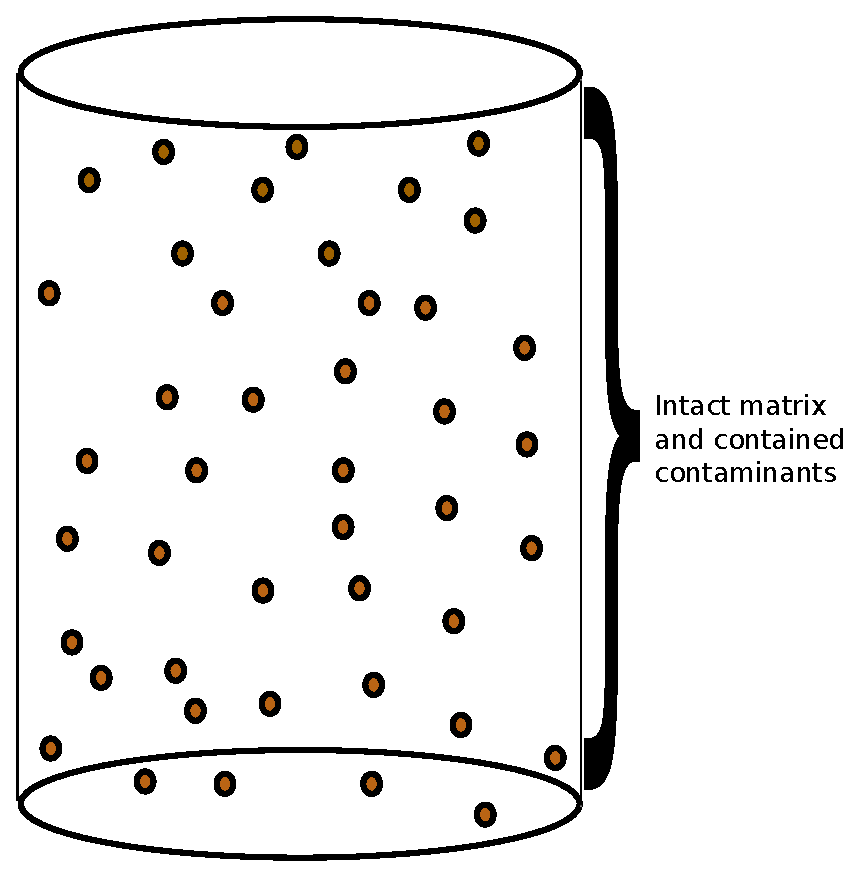
\includegraphics[height=7cm]{./chapters/nuclide_models/mixed_cell/mixed_cell_whole.eps}
  \end{center}
  \caption[Intact Mixed Cell Control Volume]{The control volume contains an 
  intact material matrix and contaminants that are unavailable to neighboring 
  subcomponents until dissolution has begun.}
  \label{fig:intact}
\end{minipage}
\hspace{0.5cm}
\begin{minipage}[b]{0.5\linewidth}
  \begin{center}
    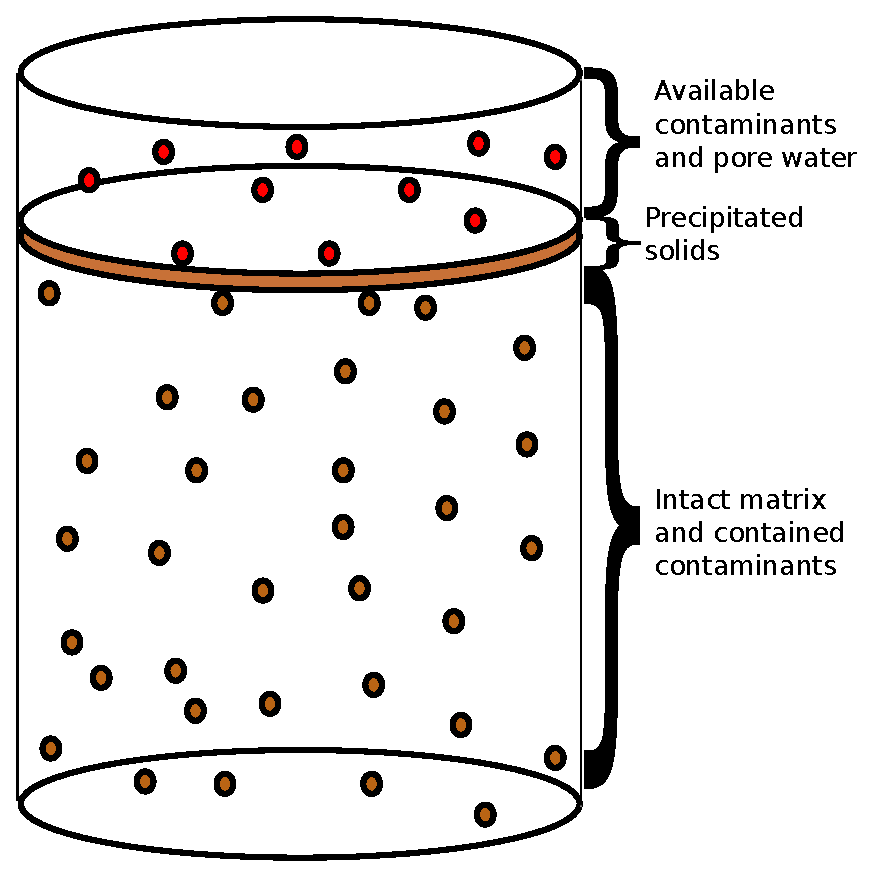
\includegraphics[height=7cm]{./chapters/nuclide_models/mixed_cell/mixed_cell_degraded.eps}
  \end{center}
  \caption[Degrading Mixed Cell Control Volume]{Once dissolution begins, the 
  :control volume contains a partially dissolved material matrix, contaminated 
  pore water, and precipitated solids.}
  \label{fig:dissolved}
\end{minipage}
\end{figure}


After some time degrading, the volume of free fluid can be expressed 
\begin{align}
V_{ff}(t_n) &= \theta V_T \int_{t_0}^{t_n} f(\cdots) dt.
\label{vff}
\end{align}

The volume of the intact matrix can be expressed
\begin{align}
V_{im}(t_n) &= V_T - V_T\int_{t_0}^{t_n} f(\cdots) dt.
\label{vim}
\end{align}

Finally, the volume of the precipitated solids can be expressed
\begin{align}
V_{ps}(t_n) &= (1 - \theta)V_T\int_{t_0}^{t_n} f(\cdots) dt.
\label{vps}
\end{align}

This model assumes that all net influx to the cell enters the free fluid rather 
than the intact matrix. The total volumetric contaminant concentration in the intact matrix, 
can be expressed

\begin{align}
C_{im}(t_n) &= C_0\\
            &= \frac{m_0}{V_{im}}
\intertext{where}
%here we assume nothing escapes an intact matrix
m_0 &= \mbox{ total initial mass } \nonumber
\end{align}

The resulting contaminant mass in the intact matrix is 

\begin{align}
m_{im}(t_n) &= C_0 V_{im}(t_n)\nonumber\\
            &= C_0(1-\theta) V_T\int_{t_0}^{t_n}f(\cdots)dt. 
\label{mim}
\end{align}

The contaminant mass in the free fluid is just the pore water concentration 
times the free fluid volume plus the time integral of net influx to the cell. 

\begin{align}
C_{ffT}(t_n) &= \left[C_0 + \frac{\int_{t_0}^{t_n} \dot{m}_{i}(t') dt'}{V_{ff}(t_n)}\right] 
\intertext{and}
m_{ffT}(t_n) &= C_{ff}(t_n)\theta V_{ff}(t_n)\nonumber\\
       &= \left[C_0 + \frac{\int_{t_0}^{t_n} \dot{m}_{i}(t') dt'}{V_{ff}(t_n)}\right] V_{ff}(t_n) \nonumber\\
       &= C_0V_{ff}(t_n) + \int_{t_0}^{t_n} \dot{m}_{i} dt'
\end{align}

It is limited, however, by both solubility limitation and sorption. 

\subsection{Sorption}

The mass in both the free fluid and in the intact matrix exists in both 
sorbed and nonsorbed phases. The relationship between the sorbed mass 
concentration in the solid phase (e.g. the pore walls),

\begin{align}
s &=\frac{\mbox{ mass of sorbed contaminant} }{ \mbox{mass of total solid phase }}
\label{solid_conc}
\end{align}
and the dissolved liquid concentration, 
\begin{align}
c &=\frac{\mbox{ mass of dissolved contaminant} }{ \mbox{volume of total liquid phase }}
\label{liquid_conc}
\end{align}
can be expressed by a number of isotherm models.

In this model, sorption is taken into account throughout the volume. In the 
intact matrix, the contaminant mass is distributed between the pore walls and 
the pore fluid by sorption.  So too, contaminant mass released from the intact 
matrix by degradation is distributed between dissolved mass in the free fluid 
and sorbed mass in the precipitated solids.


\subsection{Boundary Conditions}

To solve for the boundary condiitons in this model, the amount of dissolved mass 
in the free fluid must be found. This value, $m_{ffl}$, can be expressed in terms of the 
total degraded contaminant mass and the contaminant mass in the precipitated 
solid,

\begin{align}
m_{ffl} &= m_{ffT} - m_{psc}
\label{m_ffl}
\end{align}

The mass of contaminant sorbed into the precipitated solids can be found using a 
linear isotherm model, characterized by the relationship 
\begin{align}
s_{i} &= K_{di} c_{i}
\label{linear_iso}
\intertext{where}
s_i &= \mbox{ the solid concentration of isotope i }[kg/kg]\nonumber\\
K_{di} &= \mbox{ the distribution coefficient of isotope i}[]\nonumber\\
c_i &= \mbox{ the liquid concentration of isotope i }[kg/m^3].\nonumber
\end{align}

Thus, 

\begin{align}
s_{i,ps} &= \frac{\mbox{contaminant mass in precipitated solids} }{ \mbox{total mass of precipitated solids}}\nonumber\\
         &= \frac{m_{psc}}{m_{pst}}\nonumber\\
         &= \frac{m_{psc}}{m_{psm} + m_{psc}}\nonumber\\
\intertext{where}
m_{psm}  &= \mbox{ noncontaminant mass in precipitated solids }[kg]\nonumber\\
         &= \rho_bV_{ps}\nonumber\\
m_{psc}  &= \mbox{ contaminant mass in precipitated solids }[kg]\nonumber\\
m_{psm}  &= \rho_bV_{ps}.
\label{s_ps}
\end{align}

The following expression results, giving contaminant mass in the precipitated 
solids in terms of the sorption coefficient,
\begin{align}
m_{psc} &= s_{ps}m_{psT}\nonumber\\
          &= K_dC_{ffl}m_{psT}\nonumber\\
          &= \frac{K_dm_{ffl}m_{psT}}{V_{ff}}\nonumber\\
          &= \frac{K_d}{V_{ff}}(m_{ffT}-m_{psc})m_{psT}\nonumber\\
          &= \frac{K_d}{V_{ff}}(m_{ffT}-m_{psc})(m_{psm}+m_{psc})\nonumber\\
          &= \frac{K_d}{V_{ff}}(m_{ffT}m_{psm}-m_{psc}m_{psm} + m_{ff}m_{psc} -m_{psc}^2)\nonumber\\
          &= \frac{K_d}{V_{ff}} (m_{ffT}m_{psm} + (m_{ffT} - m_{psm})m_{psc} - m_{psc}^2)\nonumber
\intertext{which, rearranged, becomes }
0         &= m_{psc}^2 + \left( -m_{ffT} + m_{psm} + \frac{V_{ff}}{K_d} \right)m_{psc} - m_{ffT}m_{psm}\nonumber
\intertext{and is solved using the quadratic formula, such that}
m_{psc}   &= \frac{m_{ffT} - m_{psm} - \frac{V_{ff}}{K_d}}{2} \nonumber\\
          & \pm\frac{\sqrt{m_{ffT}^2 + m_{psm}^2 + \frac{V_{ff}^2}{K_d^2} + 2m_{ffT}m_{psm} - 
             \frac{2V_{ff}m_{ffT}}{K_d} + \frac{2V_{ff}m_{psm}}{K_d} } }{2} \nonumber
\intertext{which, again rearranged, becomes}
          &= \frac{1}{2} \left(m_{ffT} - m_{psm} - \frac{V_{ff}}{K_d}\right) \nonumber\\
          & \pm \frac{1}{2} \sqrt{m_{ffT}^2 + 2m_{ffT}\left(m_{psm} - 
          \frac{V_{ff}}{K_d}\right) + \left(m_{psm} + 
          \frac{V_{ff}}{K_d}\right)^2}.
\label{m_psc}
\end{align}

If we plug Equation \eqref{m_psc} into Equation \eqref{m_ffl}, we arrive at the 
following expression for $m_{ffl}$ in terms of known quantities

\begin{align}
m_{ffl}   &= m_{ffT} - \frac{1}{2} \left(m_{ffT} - m_{psm} - \frac{V_{ff}}{K_d}\right) \nonumber\\
          & \mp \frac{1}{2} \sqrt{m_{ffT}^2 + 2m_{ffT}\left(m_{psm} - 
          \frac{V_{ff}}{K_d}\right) + \left(m_{psm} + 
          \frac{V_{ff}}{K_d}\right)^2}.
\label{m_ffl_full}
\end{align}

We can express the desired boundary conditions in terms of $m_{ffl}$. First, the 
Dirichlet boundary condition is 
\begin{align}
C(x,y,z,t) = \frac{m_{ffl}(t)}{V_{ff}(t)}\forall (x,y,x) \in \Gamma.
\label{dirichlet_mixed}
\end{align}

Again, the concentration gradient can be specified across the boundary only with 
reference to the concentration at a point external to the component. 
If the concentration $C_{ext}$ is specified at a location $r_{ext}$, the Neumann 
condition is a function of those concentrations, $C(x,y,z,t)$, and a 
corresponding location inside the component. If we choose radius furthest from 
either wall of the inner component, $r_c$, 

\begin{align}
\frac{\partial C}{\partial r} = \frac{C_{ext} - C(x,y,z,t)}{r_{ext} - r_{c}}&
\label{neumann_mixed}
\intertext{such that}
\theta_i\vec{v_i}(t) C(x,y,z,t) \frac{C_{ext} - C(x,y,z,t)}{r_{ext} - r_{c}} &= \theta_i\vec{v_i}(t) C(x,y,z,t).
\end{align}





%\subsubsection{Lumped Parameter Mass Balance Model}\label{sec:lumped}
\subsubsection{Lumped Parameter Radionuclide Mass Balance Model}\label{sec:lumped}

For systems in which the flow is sufficiently slow to be assumed constant over 
a time step, it is possible to model a system of volumes as a connected lumped 
parameter models (Figure \ref{fig:lumpedseries}). 
The Lumped Parameter mass balance model implements a response function model 
based on this lumped parameter interpretation and capable of Piston Flow, 
Exponential, and Dispersion response functions from Maloszewski and Zuber 
\cite{maloszewski_lumped_1996}.

\begin{figure}[htbp!]
  \begin{center}
    \def\svgwidth{.8\textwidth}
    \input{./chapters/methodology/nuclide_models/mass_balance/lumped/lumpedseries.eps_tex}
  \end{center}
  \caption{A system of volumes can be modeled as lumped parameter models in 
  series.}
  \label{fig:lumpedseries}
\end{figure}

Each lumped parameter component is modeled according to a 
relationship between the incoming concentration, $C_{in}(t)$, and the outgoing 
concentration, $C_{out}(t)$, 

\begin{align}
  C_{out}(t) &= \int_0^\infty C_{in}(t-t')g(t')e^{-\lambda t'}dt'
  \label{lumped2}
  \intertext{where}
  t'  &= \mbox{ transit time }[s]\nonumber\\
  g(t')  &= \mbox{ response function, a.k.a. transit time distribution}[-]\nonumber]\\
  \lambda &= \mbox{ radioactive decay constant }[s^{-1}].\nonumber
\end{align}

Selection of the response function is usually based on experimental tracer 
results in the medium at hand. If such data is available, functions used 
commonly in chemical engineering applications \cite{maloszewski_lumped_1996} 
include the Piston Flow Model (PFM), 

\begin{align}
  g(t') &= \delta{(t'-t_t))}
  \intertext{ the Exponential Model (EM) }
  g(t') &= \frac{1}{t_t}e^{-\frac{t'}{t_t}}
  \intertext{ and the Dispersion Model (DM), }
  g(t') &= \left( \frac{\emph{Pe }t_t}{4\pi t'} \right)^{\frac{1}{2}}
  \frac{1}{t'}e^{- \frac{\emph{Pe }t_t\left( 1- \frac{t'}{t_t}  \right)^2} 
  {4t'}}, \intertext{where}
  \emph{Pe}  &= \mbox{ Peclet number for mass diffusion }[-]\nonumber\\
  t_t  &= \mbox{ mean tracer age }[s]\nonumber\\
    &= t_w \mbox{ if there are no stagnant areas }\nonumber\\
  t_w  &= \mbox{ mean residence time of water }[s]\nonumber\\
       &= \frac{V_m}{Q}\nonumber\\
       &= \frac{z}{v_z}\nonumber\\
       &= \frac{z\theta_e}{q}\nonumber
  \intertext{in which}
  V_m  &= \mbox{ mobile water volume }[m^3]\nonumber\\
  Q    &= \mbox{ volumetric flow rate }[m^3/s]\nonumber\\
  z    &= \mbox{ average travel distance in flow direction }[m]\nonumber\\
  v_z  &= \mbox{ mean water velocity}[m/s]\nonumber\\
  q    &= \mbox{ Darcy Flux }[m/s]\nonumber\\
  \theta_e &= \mbox{ effective (connected) porosity }[\%].\nonumber
\end{align}

The latter of these, the Dispersion Model satisfies the one dimensional 
advection-dispersion equation, and is therefore the most physically relevant for 
this application. The solutions to these for constant concentration at the 
source boundary are given in Maloszewski and Zuber \cite{maloszewski_lumped_1996}, 

\begin{align}
  C_{out}(t) &=\begin{cases}
    PFM & C_0e^{-\lambda t_t}\\
    EM  & \frac{C_0}{1+\lambda t_t}\\
    DM & C_0e^{\frac{\emph{Pe}}{2}\left(1-\sqrt{1+\frac{4\lambda 
    t_t}{\emph{Pe}}}\right)}.
  \end{cases}
  \label{lumpedsolns}
\end{align}

Since \Cyclus handles decay outside of \Cyder, the use of these models relies on a 
reference transit time and decay constant supplied by the user. The behavior of 
the reference isotope, in this way, fully defines the behavior of all isotopes.

It is important to note that a linear concentration profile is assumed between 
the inlet and the outlet,

\begin{align}
  C(z,t) = C_{in}(t)  + \frac{C_{out}(t) - C_{in}(t)}{z_{out} - z_{in}}z.
\end{align}


%\subsubsection{One Dimensional PPM Mass Balance Model}\label{sec:one_dim_ppm}
\subsection{One Dimensional Permeable Porous Medium Radionuclide Transport 
Model}\label{sec:one_dim_ppm}
Finally, abstraction results informed modifications to the implementation of an 
analytic solution to the one dimensional advection-dispersion equation with 
finite domain and Cauchy and Neumann boundary conditions at the inner and outer 
boundaries, respectively. 

Various solutions to the advection dispersion equation  
\eqref{unidirflow} have been published for both the first and third types of 
boundary conditions. The third, Cauchy type, is mass conservative, and will be 
the primary kind of boundary condition used at the source for this model.

The conceptual model in Figure \ref{fig:1dinf} represents solute transport in 
one dimension with unidirectional flow upward (a conservative assumption) and a 
semi-infinite boundary condition in the positive flow direction. The solution is 
given (Leij et. al, \cite{leij_analytical_1991}) and described below.  

\begin{figure}[h!]
  \begin{center}
    \def\svgwidth{.5\textwidth}
    \input{./chapters/methodology/nuclide_models/one_dim_ppm/1dinf.eps_tex}
  \end{center}
  \caption{A one dimensional, semi-infinite model, unidirectional flow,
  solution with Cauchy and Neumann boundary conditions}
  \label{fig:1dinf}
\end{figure}

For the boundary conditions, 
\begin{align}
  -D \frac{\partial C}{\partial z}\big|_{z=0} + v_zc &= \begin{cases}
    v_zC_0  &  \left( 0<t<t_0 \right)\\
    0  &  \left( t>t_0 \right)\\
  \end{cases},\\
  \frac{\partial C}{\partial z}\big|_{z=\infty} &= 0
  \intertext{and the initial condition,}
  C(z,0) &= C_i,
  \label{1dinfBC}
  \intertext{the solution is given as }
  C(z,t) = \frac{C_0}{2}\Bigg[&\mbox{erfc}\left[{\frac{L-v_zt}{2\sqrt{D_Lt}}}\right] 
  + \frac{1}{2} \left(\frac{v_z^2t}{\pi D_L}\right)^{1/2}e^{\frac{-( L - 
  v_zt)^2}{4D_Lt}}\nonumber\\
  &- \frac{1}{2}\left( 
  1+\frac{v_zL}{D_L}+\frac{v_z^2t}{D_L}\right)e^\frac{v_zL}{D_L}\mbox{erfc}\left[\frac{L-V_zt}{2\sqrt{D_Lt}}\right]
  \Bigg].
\end{align}





\section{Demonstration}
% Provide your results:
%       clearly

The primary outcome of this work is a mulitdimensional database of repository temperature 
change per mass of high heat contributing isotopes supporting the implementation 
of the \gls{STC} method in \Cyder. 

A validation effort concerning this tool was performed to assess the validity 
of the \gls{STC} method for the purpose of repository thermal response 
estimation.  Comparison of the results of this method with the \gls{LLNL} model 
\cite{greenberg_application_2012} gave results within the accuracy range of the 
model itself performs against the SINDA code \cite{huff_numerical_2012} and 
demonstrated the way in which inaccuracies from neglected low heat contributing 
nuclides are bounded. Details of that comparison can be found in Appendix 
\ref{ch:thermal_accuracy}. 

Figures \ref{fig:CmValidation} and \ref{fig:CmPercentError} show the results of 
one example validation exercise comparing the combined scaling and  
superposition calculations demonstrated in Figures \ref{fig:CmScaling} and 
\ref{fig:CmSuperposition} respectively. This particular validation example, 
containing no neglected nuclides, demonstrates an average error of 1.1\% and a 
maximum error of 4.4\%, where percent error is 
\begin{align}
\mbox{ percent error } &= 100\times\frac{\left|\Delta T_{LLNL} - \Delta T_{STC}\right|}{ \Delta T_{LLNL}}.
\end{align}

\begin{figure}[htp!]
\begin{center}
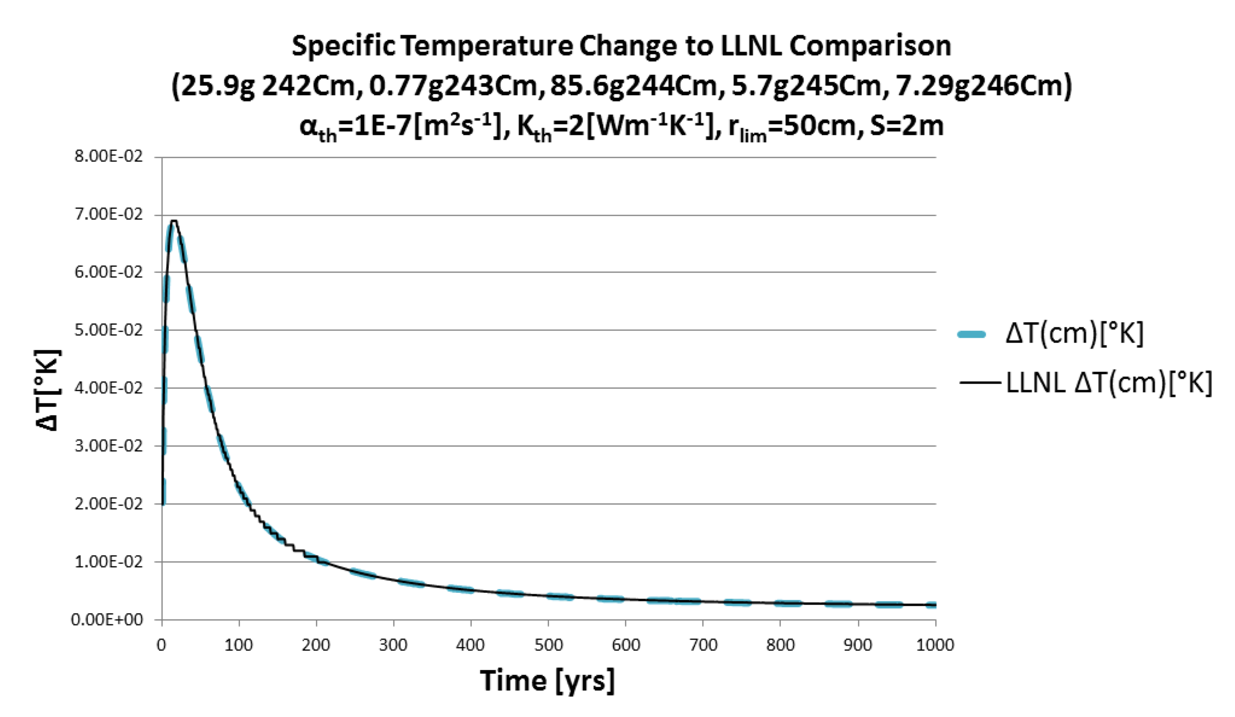
\includegraphics[width=\columnwidth]{./chapters/methodology/thermal_models/CmValidation.eps}
\end{center}
\caption{This comparison of \gls{STC} calculated thermal response from $Cm$ 
inventory per MTHM in 51GWd burnup UOX PWR fuel compares favorably with results 
from the semi-analytic model from LLNL.} 
\label{fig:CmValidation}
\end{figure}

\begin{figure}[htp!]
\begin{center}
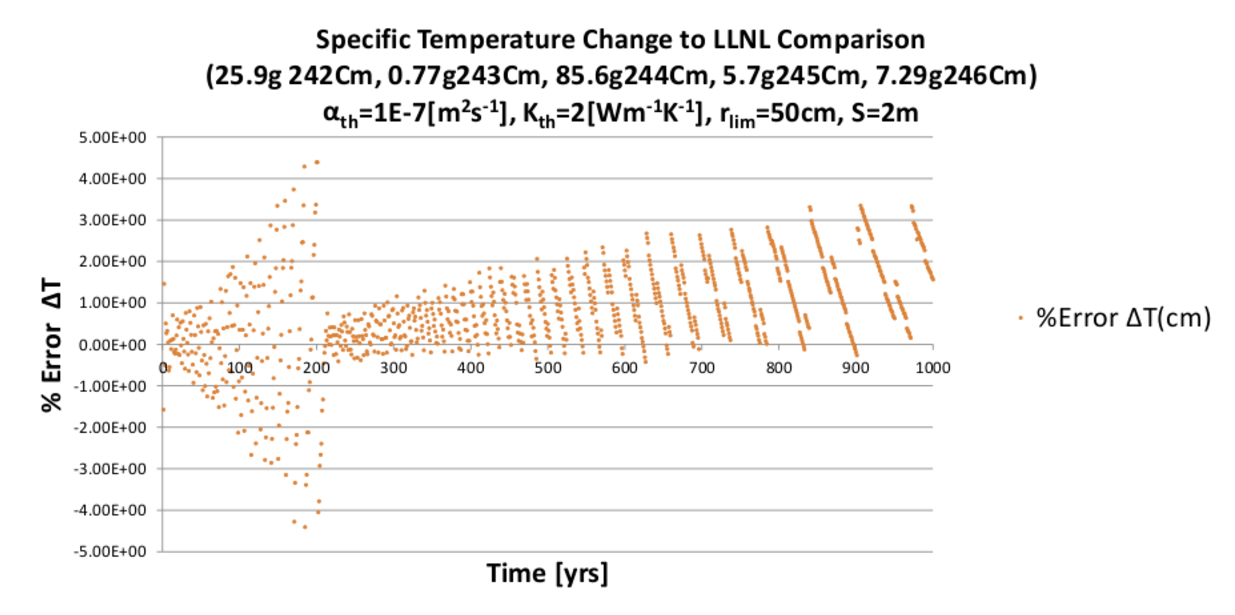
\includegraphics[width=\columnwidth]{./chapters/methodology/thermal_models/CmPercentError.eps}
\end{center}
\caption{Percent error between the semi-analytic model from LLNL and the \gls{STC} 
calculated thermal response from $Cm$ inventory per MTHM in 51GWd burnup UOX 
PWR fuel demonstrates a maximum percent error of 4.4\%.}
\label{fig:CmPercentError}
\end{figure}
% Unit Test Results
In addition to this validation effort, continual verification of code behavior 
is enabled by a suite of unit tests packaged with the tool. These tests are 
provided along with the source code so that they may be performed to evaluate 
the implementated behavior of units of functionality within the interpolation 
and specific temperature change algorithms even as the code is improved in the 
future.  

\subsection{Thermal Toy Cases}
\subsection{Radionuclide Toy Cases}
\subsection{Thermal Validation Cases}
\subsection{Radionuclide Validation Cases}

\chapter{Conclusions}\label{ch:conclusion}
\section{Contributions}

This work has provided a repository anaylsis module for fuel cycle analysis 
that is the first of its kind. That is, it provides the first generic geology 
repository model integrated dynamically within a fuel cycle simulation code.

The Cyder source code in which these models are implemented as well as 
associated documentation are freely available to interested researchers and 
potential model developers. The application programming interface to this 
software library is intentionally general, facilitating the incorporation of 
the models presented here within external software tools in need of a 
multicomponent repository model.

Furthermore, this work contributes to an expanding ecosystem of computational 
models available for use with the Cyclus fuel cycle simulator. This hydrologic 
nuclide transport library, by virtue of its capability to modularly integrate 
with the Cyclus fuel cycle simulator has laid the foundation for integrated 
disposal option analysis in the context of fuel cycle options. 

\section{Suggested Future Work}

%%--------------------------------%%
%%--------------------------------%%
\begin{frame}[allowframebreaks]
  \frametitle{References}
  \bibliographystyle{plain}
  {\footnotesize \bibliography{ne571} }

\end{frame}

%%--------------------------------%%




\end{document}



